\newpage
\section{ĐƯỜNG TRÒN TRONG MẶT PHẲNG TỌA ĐỘ}
\subsection{LÝ THUYẾT CẦN NHỚ}
\subsubsection{Phương trình đường tròn}
	Đường tròn tâm $I$, bán kính $R$ là tập hợp những điểm $M$ thoả mãn điều kiện $IM=R$.
\begin{center}
	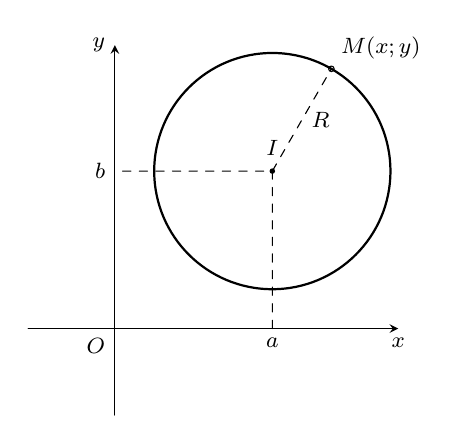
\begin{tikzpicture}[scale=1, font=\footnotesize, line join=round, line cap=round,>=stealth]
		\def\xmin{-1}
		\def\xmax{3.5}
		\def\ymin{-1}
		\def\ymax{3.5}
		\draw[->] (\xmin-0.1,0)--(\xmax+0.1,0) node[below] { $x$};
		\draw[->] (0,\ymin-0.1)--(0,\ymax+0.1) node[left] { $y$};
		\draw (0,0) node [below left] { $O$};
		\path 	(2,2) coordinate (I) (4,0)
		(2,2) arc (180:120:1.5cm) coordinate (M);
		\draw[dashed] (2,0)--(I)--(0,2) (I)--(M) node[pos=0.5,right] {$R$};
		\draw[thick] (2,2) circle (1.5cm);
		\draw 	(M) circle (1pt) node[above right] {$M(x;y)$}
		(2,0) node[below] {$a$}
		(0,2) node[left] {$b$}; 
		\foreach \p/\g in {I/90} \fill[black] (\p) circle(1pt)+(\g:0.3) node{$\p$};
	\end{tikzpicture}
\end{center}
\begin{boxdn}
	Trong mặt phẳng $Oxy$, điểm $M(x;y)$ thuộc đường tròn $(C)$, tâm $I(a;b)$, bán kính $R$ khi và chỉ khi
	\begin{align}
		\left(x-a\right)^2+\left(y-b\right)^2=R^2. \tag{1} \label{0H3-1-1}
	\end{align}
	Ta gọi \eqref{0H3-1-1} là phương trình của đường tròn $(C)$.
\end{boxdn}
\begin{note}
	Ta có thể viết phương trình đường tròn về dạng $x^2+y^2-2ax-2by+c=0$.\\
	Một phương trình có dạng $x^2+y^2-2ax-2by+c=0$ là phương trình đường tròn khi và chỉ khi $a^2+b^2-c>0$, lúc này đường tròn đó có tâm $I(a;b)$, bán kính $R=\sqrt{a^2+b^2-c}$.
\end{note}
\subsubsection{Phương trình tiếp tuyến đường tròn}
\begin{boxdn}
	Cho điểm $M\left(x_0;y_0\right)$ thuộc đường tròn $(C) \colon \left(x-a\right)^2+\left(y-b\right)^2=R^2$ (tâm $I(a;b)$, bán kính $R$). Khi đó, tiếp tuyến $\Delta$ của $(C)$ tại $M\left(x_0;y_0\right)$ có vectơ pháp tuyến $\overrightarrow{MI}=\left(a-x_0;b-y_0\right)$ và phương trình $$\left(a-x_0\right)\left(x-x_0\right)+\left(b-y_0\right)\left(y-y_0\right)=0.$$
	\begin{center}
		\begin{tikzpicture}[scale=1, font=\footnotesize, line join=round, line cap=round,>=stealth]
			\def\xmin{-1}
			\def\xmax{3.5}
			\def\ymin{-1}
			\def\ymax{3.5}
			\pgfmathsetmacro\r{sqrt(2)}
			\path 	(0,0) coordinate (I)
			(-0.5,2.5) coordinate (A)
			(3,-1) coordinate (B);
			\draw[thick,name path=tr] (0,0) circle (\r);
			\draw[thick,name path=th] (A)--(B) node[above right] {$\Delta$}; 
			\path[name intersections={of=tr and th}] (intersection-1) coordinate (M);
			\draw (I)--(M);
			\foreach \p/\g in {I/90,M/45} \fill[black] (\p) circle(1pt)+(\g:0.3) node{$\p$};
			\draw 	pic[draw,angle radius=2mm]{right angle=A--M--I};
		\end{tikzpicture}
	\end{center}
\end{boxdn}
\subsection{PHÂN LOẠI VÀ PHƯƠNG PHÁP GIẢI TOÁN}
\begin{dang}{Xác định tâm và bán kính của đường tròn cho trước}
\textbf{Phương pháp giải}
\\
Ta có hai trường hợp:
\begin{itemize}
    \item \textbf{Dạng 1: $(x-a)^2 + (y-b)^2 = R^2$}\\
    Đường tròn có tâm $I(a;b)$ và bán kính $R$.
    \item \textbf{Dạng 2: $x^2 + y^2 - 2ax - 2by + c = 0$}\\
    \textbf{Bước 1:} Kiểm tra điều kiện $a^2+b^2-c > 0$. Nếu không thỏa mãn, đây không phải phương trình đường tròn.
    \\
    \textbf{Bước 2:} Nếu thỏa mãn, đường tròn có tâm $I(a;b)$ và bán kính $R = \sqrt{a^2+b^2-c}$.
\end{itemize}
\textbf{Lưu ý:} Nếu phương trình có dạng $Ax^2+Ay^2+...=0$ ($A \neq 1$), ta phải chia cả 2 vế cho $A$ trước khi xác định $a, b, c$.
\end{dang}
\begin{vd}%[0H9N4-1]%[Dự án đề cương 3 Khối NH25-26- Đợt 2- Nguyễn Cường]
	Trong mặt phẳng $Oxy$, tìm tâm và bán kính của đường tròn có phương trình sau
\begin{multicols}{2}
		\begin{enumerate}
		\item $x^2+y^2=2$;
		\item $(x-2)^2+y^2=9$;
		\item $(x-1)^2+(y-2)^2=25$;
		\item $(x+3)^2+(y-1)^2=16$.
	\end{enumerate}
\end{multicols}
	\loigiai{
	\begin{enumerate}
		\item Đường tròn có tâm $O(0;0)$ và bán kính $R=\sqrt{2}$.
		\item Đường tròn có tâm $A(2;0)$ và bán kính $R=3$.
		\item Đường tròn có tâm $B(1;2)$ và bán kính $R=5$.
		\item Đường tròn có tâm $I(-3;1)$ và bán kính $R=4$.
	\end{enumerate}
	}
\end{vd}
\begin{vd}%[0H9N4-1]%[Dự án đề cương 3 Khối NH25-26- Đợt 2- Nguyễn Cường]
	Phương trình nào trong các phương trình sau đây là phương trình đường tròn? Tìm tọa độ tâm và bán kính của đường tròn đó.
\begin{multicols}{2}
	\begin{enumerate}
		\item $x^2+y^2 -2x-4y-20=0$;
		\item $x^2+y^2+2x-4y+6=0$;
		\item $x^2+y^2-4x-8y+5=0$;
		\item $2x^2+2y^2+6x+8y-2=0$.
	\end{enumerate}
\end{multicols}
\loigiai{
	\begin{enumerate}
		\item 
		$$	x^2+y^2 -2x-4y-20=0\quad (1)$$			
		Phương trình $(1)$ có dạng $x^2 +y^2 -2ax -2by +c=0$ với $a= 1$; $b=2$; $c=-20$.\\
		Ta có $a^2+b^2 -c=1+4+20=25>0$.\\
		Vậy $(1)$ là phương trình đường tròn có tâm $I(1;2)$ và có bán kính $R=5$.
		\item 
		$$x^2+y^2+2x-4y+6=0\quad (2)$$
		Phương trình $(2)$ có dạng $x^2 +y^2 -2ax -2by +c=0$ với $a= -1$; $b=2$; $c=6$.\\
		Ta có $a^2+b^2 -c =1+4-6=-1<0$.\\
		Vậy $(2)$ không phải là phương trình đường tròn.
		\item 
		$$x^2+y^2-4x-8y+5=0\quad (3)$$
		Phương trình $(3)$ có dạng $x^2 +y^2 -2ax -2by +c=0$ với $a= 2$; $b=4$; $c=5$.\\
		Ta có $a^2+b^2 -c =4+16-5=15>0$.\\
		Vậy $(2)$ là phương trình đường tròn tâm $I(2;4)$ và bán kính $R=\sqrt{15}$.
		\item 
		$$2x^2+2y^2+6x+8y-2=0
		\Leftrightarrow x^2 +y^2 +3x+4y-1=0\quad (4)$$	
		Phương trình $(4)$ có dạng $x^2 +y^2 -2ax -2by +c=0$ với $a= -\dfrac{3}{2}$; $b=-2$; $c=-1$.\\
		Ta có $a^2+b^2 -c =\dfrac{9}{4}+4+1=\dfrac{29}{4}>0$.\\
		Vậy $(4)$ là phương trình đường tròn tâm $I(-\dfrac{3}{2};-2)$ và bán kính $R=\dfrac{\sqrt{29}}{2}$.
	\end{enumerate}
	}
\end{vd}
\begin{vd}%[0H9H4-1]%[Dự án đề cương 3 Khối NH25-26- Đợt 2- Nguyễn Cường]
	Trong mặt phẳng $Oxy$, cho phương trình $x^2+y^2-2mx-4(m-2)y+6-m=0 \quad(1)$. Tìm điều kiện của $m$ để (1) là phương trình đường tròn.
	\loigiai{
		Phương trình (1) là phương trình đường tròn khi và chỉ khi $a^2+b^2-c > 0$, với $a=m$; $b=2(m-2)$; $c=6-m$.\\
		Hay $m^2+4(m-2)^2-6+m > 0\Leftrightarrow 5m^2-15m+10 > 0\Leftrightarrow \hoac{& m > 2 \\ & m < 1.}$
	}
\end{vd}
\begin{dang}{Lập phương trình đường tròn}
\textbf{Phương pháp giải}
\\
\textbf{Cách 1: Sử dụng phương trình dạng $(x-a)^2 + (y-b)^2 = R^2$}
\begin{itemize}
    \item \textbf{Bước 1:} Tìm tọa độ tâm $I(a;b)$.
    \item \textbf{Bước 2:} Tính bán kính $R$. (Ví dụ: $R=IM$ nếu đường tròn đi qua M, $R = d(I, \Delta)$ nếu đường tròn tiếp xúc với $\Delta$).
    \item \textbf{Bước 3:} Thay vào công thức.
\end{itemize}
\textbf{Cách 2: Sử dụng phương trình dạng $x^2 + y^2 - 2ax - 2by + c = 0$}
\begin{itemize}
    \item \textbf{Bước 1:} Giả sử phương trình có dạng trên.
    \item \textbf{Bước 2:} Dựa vào các điều kiện của bài toán (đi qua $3$ điểm, tâm thuộc đường thẳng,...) để lập một hệ phương trình $3$ ẩn $a$, $b$, $c$.
    \item \textbf{Bước 3:} Giải hệ tìm $a$, $b$, $c$ và viết phương trình.
\end{itemize}
Cách $2$ thường được dùng khi đường tròn đi qua $3$ điểm cho trước.
\end{dang}

\begin{vd}%[0H9N4-2]
	Trong mặt phẳng $Oxy$, viết phương trình của đường tròn tâm $I(-3;5)$, bán kính $R=7$.
	\loigiai{ Phương trình của đường tròn tâm $I(-3;5)$, bán kính $R=7$ là $(x+3)^2+(y-5)^2=49$.}
\end{vd}

\begin{vd}[Trích đề thi HK2-THPT Lương Ngọc Quyến-Thái Nguyên-Năm học 2024-2025]%[0H9H4-2]%[Dự án đề cương 3 Khối NH25-26- Đợt 2- Nguyễn Cường]
Trong mặt phẳng $Oxy$, viết phương trình của đường tròn $( C )$ có tâm $I( -2;3 )$ và đi qua $M( 2;-3 )$.
	\loigiai{
		Ta có $\overrightarrow{IM}=(4;-6)\Rightarrow $ bán kính $R=IM=\sqrt{4^2+(-6)^2}=\sqrt{52}.$\\
		Phương trình đường tròn $(C)$ là $(x+2)^2+(y-3)^2=52\Leftrightarrow x^2+y^2+4x-6y-39=0$.
	}
\end{vd}
\begin{vd}%[0H9H4-2]%[Dự án đề cương 3 Khối NH25-26- Đợt 2- Nguyễn Cường]
	Trong mặt phẳng $Oxy$, cho hai điểm $A(-4; -6)$ và $B(7; -1)$. Viết phương trình đường tròn $(C)$ nhận $AB$ là đường kính.
	\loigiai
	{
		Đường tròn $(C)$ có tọa độ tâm $I$ là trung điểm của đoạn thẳng $AB$ với $I=\left(\dfrac{-4+7}{2};\dfrac{-6+(-1)}{2}\right)=\left(\dfrac{3}{2};-\dfrac{7}{2}\right)$.\\
		Bán kính $R=\dfrac{AB}{2}=\dfrac{\sqrt{(7+4)^2+(-1+6)^2}}{2}=\dfrac{\sqrt{146}}{2}$.\\
		Phương trình đường tròn $(C)$ có dạng 
		$\left(x-\dfrac{3}{2}\right)^2+\left(y+\dfrac{7}{2}\right)^2=\left(\dfrac{\sqrt{146}}{2}\right)^2\Leftrightarrow \left(x-\dfrac{3}{2}\right)^2+\left(y+\dfrac{7}{2}\right)^2=\dfrac{73}{2}.$
	}
\end{vd}
\begin{vd}[Trích đề thi HK2-THPT Bình Tân-TPHCM-Năm học 2024-2025]%[0H9V4-2]%[Dự án đề cương 3 Khối NH25-26- Đợt 2- Nguyễn Cường]
	Trong mặt phẳng $Oxy$, cho $A(2;-1)$, $B(0; 5)$; $C(-3; 7)$. Tìm tọa độ tâm đường tròn ngoại tiếp tam giác $ABC$.
	\loigiai{
		Gọi $M\left(x_{M} ; y_{M}\right)$ là tâm đường tròn ngoại tiếp tam giác ${ABC}$. Ta có:
		\allowdisplaybreaks
		\begin{eqnarray*}
			\heva{&AM=BM\\&AM=CM} 
			&\Leftrightarrow& \heva{&AM^2=BM^2\\&AM^2=CM^2}\\
			&\Leftrightarrow&\heva{&\left(x_M-2\right)^2+\left(y_M+1\right)^2=x_M^2+\left(y_M-5\right)^2\\
				&\left(x_M-2\right)^2+\left(y_M+1\right)^2=\left(x_M+3\right)^2+\left(y_M-7\right)^2} \\
			&\Leftrightarrow&\heva{&-4x_{M}+12y_{M}=20\\&-10x_{M}+16y_{M}=53}\Leftrightarrow\heva{&x_M=-\dfrac{41}{7}\\&y_M=-\dfrac{2}{7}.}	
		\end{eqnarray*}
		Vậy $M\left(-\dfrac{41}{7} ;-\dfrac{2}{7}\right)$.
}\end{vd}

\begin{vd}%[0H9H4-2]%[Dự án đề cương 3 Khối NH25-26- Đợt 2- Nguyễn Cường]
	Trong mặt phẳng $Oxy$, lập phương trình đường tròn đi qua hai điểm $A(3;0)$, $B(0;2)$ và có tâm thuộc đường thẳng $d\colon x+y=0$.
	\loigiai{ 
		Gọi $I(a;-a)$ là tâm đường tròn thuộc đường thẳng $d$. Vì đường tròn đi qua hai điểm $A$, $B$ nên ta có
		\begin{eqnarray*}
			&& IA=IB\\
			&\Leftrightarrow& IA^2=IB^2\\
			&\Leftrightarrow& (3-a)^2+a^2=(-a)^2+(2+a)^2\\
			&\Leftrightarrow & 2a^2-6a+9=2a^2+4a+4\\
			&\Leftrightarrow& a=\dfrac{1}{2}.
		\end{eqnarray*}
		Suy ra tâm đường tròn $I\left(\dfrac{1}{2};-\dfrac{1}{2}\right)$, bán kính $R=IA=\sqrt{\left(3-\dfrac{1}{2}\right)^2+\left(\dfrac{1}{2}\right)^2}=\dfrac{\sqrt{26}}{2}$.\\
		Phương trình đường tròn là $\left(x-\dfrac{1}{2}\right)^2+\left(y+\dfrac{1}{2}\right)^2=\dfrac{13}{2}$. 
		
	}
\end{vd}

\begin{vd}[Trích đề thi HK2-THPT Bình Chánh- TPHCM-Năm học 2024-2025]%[0H9H4-2]%[Dự án đề cương 3 Khối NH25-26- Đợt 2- Nguyễn Cường]
	Trong mặt phẳng $Oxy$, cho điểm $I(1;1)$ và đường thẳng $d\colon 3x+4y-2=0$. Viết phương trình đường tròn tâm $I$ và tiếp xúc với đường thẳng $d$.
	\loigiai{Bán kính đường tròn là 
		\begin{align*}
			R=\mathrm{d}(I,d)=\dfrac{\left|3\cdot1+4\cdot1-2 \right|}{\sqrt{3^2+4^2}}=1.	
		\end{align*}		
		Đường tròn tâm $I$ và tiếp xúc với đường thẳng $d$ có phương trình là 
		\begin{align*}
			(x-1)^2+(y-1)^2=1.	
	\end{align*}}
\end{vd}
\begin{dang}{Lập phương trình tiếp tuyến của đường tròn}
\textbf{Phương pháp giải}
\\
Tiếp tuyến $\Delta$ của đường tròn $(C)$ tâm $I$ là đường thẳng chỉ có một điểm chung với $(C)$. Điều kiện tương đương: $d(I, \Delta) = R$.
\begin{itemize}
    \item \textbf{Dạng 1: Viết tiếp tuyến tại điểm $M_0(x_0; y_0) \in (C)$}\\
    Tiếp tuyến $\Delta$ đi qua $M_0$ và nhận $\overrightarrow{IM_0}$ làm VTPT.
    Phương trình: $(x_I-x_0)(x-x_0) + (y_I-y_0)(y-y_0) = 0$.
    \item \textbf{Dạng 2: Viết tiếp tuyến song song hoặc vuông góc với một đường thẳng cho trước}\\
    \textbf{Bước 1:} Dựa vào điều kiện song song/vuông góc để xác định dạng phương trình của tiếp tuyến $\Delta$ (thường có $1$ tham số $m$).
    \\
    \textbf{Bước 2:} Sử dụng điều kiện $d(I, \Delta) = R$ để giải phương trình tìm $m$.
\end{itemize}
\end{dang}

\begin{vd}%[0H9H4-3]%[Dự án đề cương 3 Khối NH25-26- Đợt 2- Nguyễn Cường]
	Trong mặt phẳng $Oxy$, viết phương trình tiếp tuyến của đường tròn $x^2+y^2-2x-4y-4=0$ tại điểm $A(1;5)$.
	\loigiai{
		Thay tọa độ điểm $A$ vào phương trình đường tròn ta có $1^2+5^2-2\cdot1 -4\cdot5-4=0$.\\
		Suy ra điểm $A$ thuộc đường tròn.\\
		Từ phương trình đường tròn, ta có tâm $I(1;2)$.\\
		Phương trình tiếp tuyến của đường tròn có dạng
		\allowdisplaybreaks
		\begin{eqnarray*}
			(1-1)(x-1)+(5-2)(y-5)&=&0\\
			y-5 &=& 0.
		\end{eqnarray*}
	}
\end{vd}

\begin{vd}[Trích đề thi HK2-THPT Nguyễn Văn Cừ- Hà Nội-Năm học 2024-2025]%[0H9H4-3]%[Dự án đề cương 3 Khối NH25-26- Đợt 2- Nguyễn Cường]
	Trong mặt phẳng $Oxy$, cho hai điểm $A(1;1)$ và $B(7;5)$ và đường tròn $(C)$ nhận $AB$ là đường kính. Viết phương trình tiếp tuyến của đường tròn $(C)$ tại điểm $M(6;6)$.
	\loigiai{
		Gọi $I$ là tâm đường tròn $(C)$ có $AB$ là đường kính, do đó $I$ là trung điểm $AB$. Suy ra $I(4;3)$.\\
		Bán kính đường tròn $(C)$ là $R=AI=\sqrt{(4-1)^2+(3-1)^2}=\sqrt{13}$.\\
		Ta có $IM=\sqrt{(6-4)^2+(6-3)^2}=\sqrt{13}$, suy ra $M\in(C)$.\\
		Phương trình tiếp tuyến của đường tròn $(C)$ tại điểm $M(6;6)$ là
		\begin{eqnarray*}
			(6-4)(x-6)+(6-3)(y-6)&=&0 \\
			2x+3y-30&=&0.
		\end{eqnarray*}
	}
\end{vd}
\begin{vd}%[0H9V4-3]%[Dự án đề cương 3 Khối NH25-26- Đợt 2- Nguyễn Cường]
	Trong mặt phẳng $Oxy$, cho đường tròn $(C)\colon x^2+y^2+2x-6y+5=0$. Viết phương trình tiếp tuyến của $(C)$ song song với đường thẳng $d\colon x+2y-15=0$.
	\loigiai{
		Đường tròn $(C)$ có tâm $I(-1;3)$ và bán kính $R=\sqrt{1+9-5}=\sqrt{5}$.\\
		Tiếp tuyến $\Delta \parallel d$ nên phương trình $\Delta$ có dạng $x+2y+m=0;\,m \neq-15$.\\
		Ta có $\Delta$ là tiếp tuyến của $(C)$ khi và chỉ khi 
		\begin{eqnarray*}
			\mathrm{d}(I,\Delta)=R&\Leftrightarrow& \dfrac{|-1+6+m|}{\sqrt{1+4}}=\sqrt{5}\\  &\Leftrightarrow& |m+5|=5\\
			&\Leftrightarrow&\hoac{&m+5=-5\\&m+5=5}\\
			&\Leftrightarrow&\hoac{&m=-10\\&m=0.}
		\end{eqnarray*}
		Đối chiếu với điều kiện, ta có hai phương trình tiếp tuyến của $(C)$ là $x+2y=0$ và $x+2y-10=0$.
	}
\end{vd}
\begin{dang}{Ứng dụng}
	Bài toán thực tế.
\end{dang}

\begin{vd}%[0H9H4-7]%[Dự án đề cương 3 Khối NH25-26- Đợt 2- Nguyễn Cường]
	Thiết kế khu vườn Hạnh Phúc hình vuông cạnh $10$ m như hình vẽ
	\begin{center}
		\begin{tikzpicture}[>=stealth,line join=round,line cap=round,font=\footnotesize,scale=.5,declare function={r=5;}]
			\begin{scope}[xshift={3.5cm}]
				\draw[fill=green] (0,0)circle(r);
				\draw[fill=white] (3,0)circle(2);
				\draw[fill=white] (-2,0)circle(3);
				\draw (-5,-5)--(-5,5)--(5,5)--(5,-5)--(-5,-5);
				\draw[fill=red] (1,3) node [right] {Cỏ};			
			\end{scope}
			%	\path (current bounding box.south) node[below]{Hình $3$};
		\end{tikzpicture}
	\end{center}
	Phần được tô đậm dùng để trồng cỏ, phần còn lại lát gạch. Biết mỗi mét vuông trồng cỏ chi phí $100$ nghìn đồng, mỗi mét vuông lát gạch chi phí $300$ nghìn đồng. Khi diện tích phần lát gạch là nhỏ nhất thì tổng chi phí thi công vườn hoa Hạnh Phúc bằng xắp xỉ $x$ triệu. Tìm $x$.
	\loigiai{
		\begin{center}
			\begin{tikzpicture}[>=stealth,line join=round,line cap=round,font=\footnotesize,scale=.5,declare function={r=5;}]
				\begin{scope}[xshift={3.5cm}]
					\draw[fill=green] (0,0)circle(r);
					\draw[fill=white] (3,0)circle(2);
					\draw[fill=white] (-2,0)circle(3);
					\draw (-5,-5)--(-5,5)--(5,5)--(5,-5)--(-5,-5);
					\draw[fill=red] (1,3) node [right] {Cỏ};			
				\end{scope}
				%	\path (current bounding box.south) node[below]{Hình $3$};
			\end{tikzpicture}
		\end{center}
		Gọi $x$, $y$ (m) lần lượt là bán kính của phần lát gạch hình tròn $(x, y > 0)$ ta có $x+y=5$.\\
		Gọi $S$ (m$^2$) là phần diện tích được lát gạch của khu vườn $(S> 0)$, ta có
		$$
		S=100-25 \pi+\pi x^2+\pi y^2=100+\pi\left(x^2+y^2-25\right) \Leftrightarrow x^2+y^2=\dfrac{S+25 \pi-100}{\pi}.$$
		Ta có $(C)\colon x^2+y^2=\dfrac{S+25\pi-100}{\pi}$ có tâm $O(0; 0)$, bán kính $R=\sqrt{\dfrac{S+25\pi-100}{\pi}}$ và đường thẳng $\Delta\colon x+y-5=0$.\\
		Khi đó bài toán trở thành: Tìm $R$ nhỏ nhất để $(C)$ và $\Delta$ có ít nhất một điểm chung, với hoành độ và tung độ đều là các số dương.\\
		Ta có $(C)$ và $\Delta$ có ít nhất một điểm chung khi và chỉ khi
		$$R\ge \mathrm{d}(O, \Delta) \Leftrightarrow \sqrt{\dfrac{S+25\pi-100}{\pi}} \ge \dfrac{5}{\sqrt{2}} \Leftrightarrow S+25\pi-100\ge \dfrac{25\pi}{2} \Leftrightarrow S\ge 100-\dfrac{25\pi}{2}.$$
		Vậy diện tích phần lát gạch nhỏ nhất bằng $S_{\min}=100-\dfrac{25\pi}{2}$.\\
		Từ đó chi phí để thi công khu vườn Hạnh phúc là $100\cdot\left(100-S_{\min}\right)+300\cdot S_{\min}=22\,146$ nghìn đồng.
	}
\end{vd}

\begin{vd}%[0H9V4-7]%[Dự án đề cương 3 Khối NH25-26- Đợt 2- Nguyễn Cường]
	\immini{Ném đĩa là một môn thể thao thi đấu trong Thế vận hội Olympic mùa hè. Khi thực hiện cú ném, vận động viên thường quay lưng lại với hướng ném, sau đó xoay ngược chiều kim đồng hồ một vòng rưỡi của đường tròn để lấy đà rồi thả tay ra khỏi đĩa. Giả sử đĩa chuyển động trên một đường tròn tâm $I\left(0;\dfrac{3}{2}\right)$ bán kính $0{,}8$ trong mặt phẳng $Oxy$, (đơn vị trên hai trục là mét). Đến điểm $M\left(\dfrac{\sqrt{39}}{10};2\right)$, đĩa được ném đi (hình bên). Trong những giây đầu tiên ngay sau khi được ném đi, quỹ đạo chuyển động của chiếc đĩa có phương trình như thế nào?
	}
	{
		\begin{tikzpicture}[>=stealth,line join=round,line cap=round,font=\footnotesize,scale=1,xscale=0.8, yscale=0.8]
			\draw[->] (-3,0)--(3,0) node[below]{$x$};
			\draw[->] (0,-1)--(0,5.5) node[left]{$y$};
			\coordinate (O) at (0,0);
			\coordinate (I) at (0,1.5);
			\coordinate (M) at (0.624,2);
			\coordinate (a) at ($(M)!4!-90:(I)$);
			\draw (I) circle(0.8 cm) (M)--(a);
			\draw[fill=black]
			(I) circle(1pt) node[left]{$I$}
			(0,2) circle(1pt) node[left]{$2$}
			(M) circle(1pt) node[above]{$M$}
			(a) circle(1pt)
			($(a)+(-0.3,0.2)$) circle(1pt)
			($(a)+(-0.6,0.4)$) circle(1pt)
			($(a)+(-0.8,0.5)$) circle(1pt)
			;
		\end{tikzpicture}
	}
	\loigiai{
		Xét đường tròn $(C)$ tâm $I\left(0;\dfrac{3}{2}\right)$, bán kính $R=0{,}8$.\\
		Ta có $IM=\sqrt{\left(\dfrac{\sqrt{39}}{10}-0\right)^2+\left(2-\dfrac{3}{2}\right)^2}=0{,}8$.\\
		Suy ra điểm $M$ thuộc đường tròn tâm $I$, bán kính $R=0{,}8$.\\
		Trong những giây đầu tiên sau khi ném đi, quỹ đạo chuyển động của chiếc đĩa là một đường thẳng có phương trình là phương trình tiếp tuyến của đường tròn tại điểm $M\left(\dfrac{\sqrt{39}}{10};2\right)$
		$$\left(\dfrac{\sqrt{39}}{10}-0\right)\left(x-\dfrac{\sqrt{39}}{10}\right)+\left(2-\dfrac{3}{2}\right)(y-2)=0\Leftrightarrow\dfrac{\sqrt{39}}{10}x+\dfrac{1}{2}y+\dfrac{261}{100}=0.$$
	}
\end{vd}
\begin{vd}%[0H9C4-7]%[Dự án đề cương 3 Khối NH25-26- Đợt 2- Nguyễn Cường]
	\immini{Ông An có một mảnh đất hình vuông diện tích $100$ m$^2$. Ông muốn chia làm $3$ phần, một nửa mảnh đất là để xây nhà $(ABFE)$, phần còn lại trồng rau và hoa, trong đó phần trồng hoa là một hình tròn tiếp xúc với cạnh $EF$, cạnh $CD$ và đường đi $DO$ (như hình vẽ). Xác định vị trí tâm của phần đất trồng hoa.}
	{
		\begin{tikzpicture}[scale=1, line join=round, line cap=round, >=stealth, font=\footnotesize]
			\def\a{3};
			\pgfmathsetmacro\b{(\a/2*sqrt(2)+\a/2)/2};
			\path 
			(0:0) coordinate (D) (\a,0) coordinate (C) (\a,\a) coordinate (B) (0,\a) coordinate (A)
			(0,\a/2) coordinate (E) (\a,\a/2) coordinate (F) (\a/2,\a/2) coordinate (O) (\b,\a/4) coordinate (I);
			\draw (A)--(B)--(C)--(D)--(A) (E)--(F) (B)--(D);
			\draw (I) circle (\a/4);
			\foreach \i/\g in {A/145, B/90, C/-90, D/-145, E/180, F/0, O/90, I/-90}{
				\draw ($(\i)+(\g:3mm)$) node{$\i$};\fill[black] (\i) circle(1pt);
			}	
		\end{tikzpicture}
	}
	\loigiai{
		Chọn hệ trục tọa độ $Dxy$ như hình vẽ.
		\begin{center}
			\begin{tikzpicture}[scale=1, line join=round, line cap=round, >=stealth, font=\footnotesize]
				\def\a{3};
				\pgfmathsetmacro\b{(\a/2*sqrt(2)+\a/2)/2};
				\path 
				(0:0) coordinate (D) (\a,0) coordinate (C) (\a,\a) coordinate (B) (0,\a) coordinate (A)
				(0,\a/2) coordinate (E) (\a,\a/2) coordinate (F) (\a/2,\a/2) coordinate (O) (\b,\a/4) coordinate (I);
				\draw (A)--(B)--(C)--(D)--(A) (E)--(F) (B)--(D);
				\foreach \i/\g in {A/145, B/90, C/-90, D/-145, E/180, F/0, O/90, I/-90}{
					\draw ($(\i)+(\g:3mm)$) node{$\i$};\fill[black] (\i) circle(1pt);
				}
				\draw[->] (C)--(\a+1,0)node[above]{$x$};
				\draw[->] (A)--(0,\a+1)node[left]{$y$};
				\draw (I) circle (\a/4);
			\end{tikzpicture}	
		\end{center}
		Khi đó $D(0;0)$, $A(0;10)$, $B(10;10)$, $C(10;0)$, $E(0;5)$ và $F(10;5)$.\\
		Đường thẳng $BD$ có phương trình là $x-y=0$. Đường tròn tâm $I$ tiếp xúc với $DC$ và $EF$ nên có bán kính $R=\dfrac{5}{2}$ và $I$ có tung độ bằng $\dfrac{5}{2}$.\\
		Gọi tọa độ $I\left(a; \dfrac{5}{2}\right)$ với $0<a<10$. Ta có
		$$\mathrm{d}(I, BD)=\dfrac{5}{2} \Leftrightarrow \dfrac{\left|a-\dfrac{5}{2}\right|}{\sqrt{2}}=\dfrac{5}{2} \Leftrightarrow \hoac{&a=\dfrac{5\sqrt{2}}{2}+\dfrac{5}{2} \text{ (nhận)}\\&a=\dfrac{5}{2}-\dfrac{5\sqrt{2}}{2} \text{ (loại)}.}$$
		Vậy vị trí tâm của phần đất trồng hoa (hay tọa độ tâm $I$) là $I\left(\dfrac{5\sqrt{2}}{2}+\dfrac{5}{2}; \dfrac{5}{2}\right)$.
	}
\end{vd}
%-----------------------------------------------------------------------------
\subsection{Bài tập rèn luyện}
\ind{PHẦN I.} \inden{Câu trắc nghiệm nhiều phương án lựa chọn. Mỗi câu hỏi học sinh chỉ chọn một phương án.}\\
\setcounter{ex}{0}
\Opensolutionfile{ans}[ans/OH9-Bai3-TN]%--Đặt tên OH9-Bai3-Dang1-TN
\begin{ex}[Trích đề thi HK2-THPT Chuyên Quốc Học Huế-Năm học 2023-2024]%[0H9N4-1]%[Dự án đề cương 3 Khối NH25-26- Đợt 2- Nguyễn Cường]
	Trong mặt phẳng $Oxy$, phương trình nào dưới đây là phương trình của một đường tròn?
	\choice
	{$x^2+y^2-4 x+7=0$}
	{$x^2+y^2-2 x y-2 y+4=0$}
	{\True $x^2+y^2+3 x-2 y+1=0$}
	{$x^2+y^2+x+y+2=0$}
	\loigiai{
		Ta có $x^2+y^2+3 x-2 y+1=0 \Leftrightarrow \left (x+\dfrac{3}{2}\right )^2+\left (y-1\right )^2=\dfrac{9}{4}$. \\
		Suy ra phương trình $x^2+y^2+3 x-2 y+1=0$ là phương trình của một đường tròn.
	}
\end{ex}
\begin{ex}[Trích đề thi HK2-THPT Nguyễn Thái Bình-TPHCM-Năm học 2024-2025]%[0H9N4-1]%[Dự án đề cương 3 Khối NH25-26- Đợt 2- Nguyễn Cường]
	Trong mặt phẳng $Oxy$, cho đường tròn $(C)\colon (x+8)^2+(y-4)^2=25$. Khẳng định nào dưới đây đúng?
	\choice
	{$(C)$ có tâm $I(8;-4)$, bán kính $R=5$}
	{$(C)$ có tâm $I(8;-4)$, bán kính $R=25$}
	{\True $(C)$ có tâm $I(-8;4)$, bán kính $R=5$}
	{$(C)$ có tâm $I(-8;4)$, bán kính $R=25$}
	\loigiai{
		Đường tròn $(C)$ có tâm $I(-8;4)$, bán kính $R=5$.
	}
\end{ex}
\begin{ex}[Trích đề thi HK2-THPT Chuyên Quốc Học Huế-Năm học 2024-2025]%[0H9N4-1]%[Dự án đề cương 3 Khối NH25-26- Đợt 2- Nguyễn Cường]
	Trong mặt phẳng $Oxy$, cho đường tròn có phương trình $x^2+y^2-2 x+6 y+1=0$. Xác định toạ độ tâm $I$ của đường tròn.
	\choice
	{$I(2 ;-6)$}
	{$I(-1 ; 3)$}
	{$I(-2 ; 6)$}
	{\True $I(1 ;-3)$}
	\loigiai{
		Đường tròn $x^2+y^2-2 x+6 y+1=0$ có tọa độ tâm $I(1;-3)$.
	}
\end{ex}

\begin{ex}[Trích đề thi HK2-THPT Chuyên Lê Quý Đôn-Ninh Thuận-Năm học 2024-2025]%[0H9N4-1]%[Dự án đề cương 3 Khối NH25-26- Đợt 2- Nguyễn Cường]
	Trong mặt phẳng $Oxy$, tọa độ tâm $I$ và bán kính $R$ của đường tròn $(C)\colon x^2+y^2-5y=0$ là 
	\choice
	{$I(0;5)$, $R=5$}
	{$I(0;-5)$, $R=5$}
	{\True $I\left(0;\dfrac{5}{2}\right)$, $R=\dfrac{5}{2}$}
	{$I\left(0;-\dfrac{5}{2}\right)$, $R=\dfrac{5}{2}$}
	\loigiai{
		Ta có $\heva{&a=0\\&b=\dfrac{5}{2}\\&c=0}$. 
		Suy ra tọa độ tâm $I\left(0;\dfrac{5}{2}\right)$, bán kính $R=\sqrt{0^2+\left(\dfrac{5}{2}\right)^2-0}=\dfrac{5}{2}$.
	}
\end{ex}
\begin{ex}[Trích đề thi HK2-THPT Nguyễn Khuyến-Bình Dương-Năm học 2024-2025]%[0H9H4-1]%[Dự án đề cương 3 Khối NH25-26- Đợt 2- Nguyễn Cường]
	Trong mặt phẳng $Oxy$, tìm giá trị của $m$ để phương trình $x^2+y^2+2x+3m=0$ là phương trình của đường tròn có bán kính bằng $2$.
	\choice
	{\True $m=-1$}
	{$m=\dfrac{1}{3}$}
	{$m=1$}
	{$m=-\dfrac{1}{3}$}
	\loigiai{
		Phương trình $x^2+y^2+2x+3m=0$ có dạng $ x^2+y^2-2ax-2by+c=0$.\\ Trong đó $a=-1$, $b=0$, $c=3m$.\\
		Điều kiện để phương trình đã cho là phương trình đường tròn có bán kính bằng $2$ là
		$$a^2+b^2-c=4\Leftrightarrow 1-3m=4\Leftrightarrow m=-1.$$
	}
\end{ex}
\begin{ex}[Trích đề thi HK2-THPT Tân Túc, TPHCM-Năm học 2024-2025]%[0H9H4-1]%[Dự án đề cương 3 Khối NH25-26- Đợt 2- Nguyễn Cường]
	Trong mặt phẳng $Oxy$, đường tròn $x^2+y^2-10y-24=0$ có đường kính bằng bao nhiêu?
	\choice
	{\True $14$}
	{$\sqrt{29}$}
	{$7$}
	{$49$}
	\loigiai{
		Đường tròn $x^2+y^2-10y-24=0$ có $-2a=0$, $-2b=-10$ và $c=-24$.\\
		Suy ra $a=0$, $b=5$ nên đường tròn có tâm $I(0;5)$ và bán kính $R=\sqrt{0^2+5^2-(-24)}=7$. \\
		Do đó đường tròn trên có đường kính bằng $14$.
	}
\end{ex}
\begin{ex}[Trích đề thi HK2-THPT Chu Văn An- Hà Nội-Năm học 2024-2025]%[0H9H4-1]%[Dự án đề cương 3 Khối NH25-26- Đợt 2- Nguyễn Cường]
	Trong mặt phẳng $Oxy$, phương trình $x^2+y^2-2x+2y+m=0$ là phương trình đường tròn khi và chỉ khi
	\choice
	{\True $m<2$}
	{$m<0$}
	{$m>2$}
	{$m>0$}
	\loigiai{
		Ta có $a=1$, $b=-1$, $c=m$.\\
		Phương trình $x^2+y^2-2x+2y+m=0$ là phương trình đường tròn khi và chỉ khi
		\[a^2+b^2-c>0\Leftrightarrow 1^2+(-1)^2-m>0\Leftrightarrow m<2.\]
	}
\end{ex}
\begin{ex}[Trích đề thi HK2-THPT Trần Phú, TP.HCM-Năm học 2024-2025]%[0H9N4-2]%[Dự án đề cương 3 Khối NH25-26- Đợt 2- Nguyễn Cường]
	Trong mặt phẳng $Oxy$, phương trình đường tròn $(C)$ có tâm $I(-2; 3)$ và bán kính bằng $\sqrt{52}$ là
	\choice
	{\True $(x+2)^2+(y-3)^2=52$}
	{$(x-2)^2+(y+3)^2=\sqrt{52}$}
	{$(x+2)^2+(y-3)^2=\sqrt{52}$}
	{$(x-2)^2+(y+3)^2=52$}
	\loigiai{
		Phương trình đường tròn $(C)$ có tâm $I(-2; 3)$ và bán kính $=\sqrt{52}$ là
		$$(x+2)^2+(y-3)^2=52.$$
	}
\end{ex}
\begin{ex}[Trích đề thi HK2-THPT Lương Ngọc Quyến-Thái Nguyên-Năm học 2024-2025]%[0H9H4-2]%[Dự án đề cương 3 Khối NH25-26- Đợt 2- Nguyễn Cường]
	Trong mặt phẳng $Oxy$, đường tròn $( C )$ có tâm $I( -2;3 )$ và đi qua $M( 2;-3 )$ có phương trình là
	\choice
	{\True $x^2+y^2+4x-6y-39=0$}
	{$( x-2 )^2+( y+3 )^2=52$}
	{$( x+2 )^2+(y-3)^2=\sqrt{52}$}
	{$x^2+y^2+4x-6y-57=0$}
	\loigiai{
		Ta có $\overrightarrow{IM}=(4;-6)\Rightarrow $ bán kính $R=IM=\sqrt{4^2+(-6)^2}=\sqrt{52}.$\\
		Phương trình đường tròn $(C)$ là $(x+2)^2+(y-3)^2=52\Leftrightarrow x^2+y^2+4x-6y-39=0$.
	}
\end{ex}
\begin{ex}[Trích đề thi HK2-THPT Nguyễn Thái Bình-TPHCM-Năm học 2024-2025]%[0H9H4-2]%[Dự án đề cương 3 Khối NH25-26- Đợt 2- Nguyễn Cường]
	Trong mặt phẳng $Oxy$, phương trình đường tròn có tâm $I(3; 2)$ và đi qua điểm $B(7;4)$ là
	\choice
	{$(x+3)^2+(y+2)^2=20$}
	{$(x-3)^2+(y-2)^2=2 \sqrt{5}$}
	{\True $(x-3)^2+(y-2)^2=20$}
	{ $(x+3)^2+(y+2)^2=2 \sqrt{5}$}
	\loigiai{
		$(C)$ có tâm $I(3;2)$ và đi qua điểm $B(7;4)$ suy ra $(C)$ có bán kính $R=IB=\sqrt{16+4}=2\sqrt{5}$.\\
		Vậy $(C)$ có phương trình $(x-3)^2+(y-2)^2=20$.
	}
\end{ex}
\begin{ex}[Trích đề thi HK2-THPT Lê Quý Đôn-TPHCM-Năm học 2024-2025]%[0H9H4-2]%[Dự án đề cương 3 Khối NH25-26- Đợt 2- Nguyễn Cường]
	Trong mặt phẳng $Oxy$, cho hai điểm $A(5;-1)$, $B(-3;7)$. Đường tròn có đường kính $AB$ có phương trình là
	\choice
	{\True $x^2+y^2-2x-6y-22=0$}
	{$x^2+y^2-2x-6y+22=0$}
	{$x^2+y^2-2x-y+1=0$}
	{$x^2+y^2+6x+5y+1=0$}
	\loigiai{
		Đường tròn đường kính $AB$ có tâm $I$ là trung điểm của đoạn thẳng $AB$ và bán kính $R=\dfrac{AB}{2}$.\\
		Tâm $I(1;3)$, $R=\dfrac{\sqrt{(-3-5)^2+(7+1)^2}}{2}=4\sqrt{2}$.\\
		Phương trình đường tròn đường kính $AB$ là
		$$(x-1)^2+(y-3)^2=\left( 4\sqrt{2}\right)^2 \Leftrightarrow x^2+y^2-2x-6y-22=0.$$
	}
\end{ex}
\begin{ex}[Trích đề thi HK2-THPT Nguyễn Thái Bình-TPHCM-Năm học 2024-2025]%[0H9H4-2]%[Dự án đề cương 3 Khối NH25-26- Đợt 2- Nguyễn Cường]
	Trong mặt phẳng $Oxy$, cho tam giác vuông $OAB$ với $A(4 ; 0)$ và $B(0 ; 6)$. Phương trình đường tròn đi qua ba điểm $O$, $A$, $B$ là
	\choice
	{$(x+2)^2+(y+3)^2=13$}
	{$(x-2)^2+(y-3)^2=\sqrt{13}$}
	{$x^2+y^2+4 x+6 y=0$}
	{\True $x^2+y^2-4 x-6 y=0$}
	\loigiai{
		Gọi $I$ là trung điểm của $AB$ thì $I(2;3)$.\\ Vì tam giác $OAB$ vuông tại $O$ nên đường tròn ngoại tiếp tam giác $OAB$ có tâm là trung điểm $I$ của $AB$ và bán kính $R=\dfrac{AB}{2}=OI=\sqrt{13}.$\\
		Vậy phương trình đường tròn đi qua ba điểm $O$, $A$, $B$ là $$(x-2)^2+(y-3)^2=13\Leftrightarrow x^2+y^2-4 x-6 y=0.$$}
\end{ex}

\begin{ex}%[0H9H4-2]%[Dự án đề cương 3 Khối NH25-26- Đợt 2- Nguyễn Cường]
	Trong mặt phẳng $Oxy$, cho tam giác $A B C$ có $A(1 ;-2)$, $B(1 ; 2)$ và $C(5 ; 2)$. Phương trình đường tròn ngoại tiếp tam giác $A B C$ là
	\choice
	{$x^2+y^2-3 x+2 y+1=0$}
	{$x^2+y^2-3 x+1=0$}
	{$x^2+y^2-6 x-1=0$}
	{\True $x^2+y^2-6 x+1=0$}
	\loigiai{
		Gọi phương trình đường tròn có dạng $(C)\colon x^2+y^2-2ax-2by+c=0$.\\
		Vì $A$, $B$, $C\in(C)$.\\ 
		Ta có $\heva{&-2a+4b+c=-5\\&-2a-4b+c=-5\\&-10a-4b+c=-29}\Rightarrow\heva{&x=3\\&y=0\\&z=1.}$\\
		Vậy phương trình đường tròn là $(C)\colon x^2+y^2-6x+1=0$.	
	}
\end{ex}
\begin{ex}[Trích đề thi HK2-THPT Tân Túc, TPHCM-Năm học 2024-2025]%[0H9H4-2]%[Dự án đề cương 3 Khối NH25-26- Đợt 2- Nguyễn Cường]
	Trong mặt phẳng $Oxy$, đường tròn nào sau đây tiếp xúc với trục $Ox$?
	\choice
	{$x^2+y^2-10x=0$}
	{$x^2+y^2-5=0$}
	{$x^2+y^2-10x-2y+1=0$}
	{\True $x^2+y^2+6x+5y+9=0$}
	\loigiai{
		Xét đường tròn $x^2+y^2+6x+5y+9=0$.\\
		Ta có $-2a=6$, $-2b=5$ và $c=9$, suy ra $a=3$, $b=-\dfrac{5}{2}$ nên có tâm $I\left(-3;-\dfrac{5}{2}\right)$ và bán kính $R=\dfrac{5}{2}$. \\
		Khi đó $R=|b|=\dfrac{5}{2}$ nên đường tròn $x^2+y^2+6x+5y+9=0$ tiếp xúc với trục $Ox$.
	}
\end{ex}
\begin{ex}[Trích đề thi HK2-THPT Bình Chánh-TPHCM-Năm học 2024-2025]%[0H9H4-2]%[Dự án đề cương 3 Khối NH25-26- Đợt 2- Nguyễn Cường]
	Trong mặt phẳng $Oxy$, cho điểm $I(1;1)$ và đường thẳng $d\colon 3x+4y-2=0$. Đường tròn tâm $I$ và tiếp xúc với đường thẳng $d$ có phương trình là
	\choice
	{$(x-1)^2+(y-1)^2=5$}
	{\True $(x-1)^2+(y-1)^2=1$}
	{$(x-1)^2+(y-1)^2=25$}
	{$(x-1)^2+(y-1)^2=\dfrac{1}{5}$}
	\loigiai{
		Gọi $R$ là bán kính đường tròn tâm $I$.\\
		Đường tròn tâm $I$ và tiếp xúc với đường thẳng $d$ khi và chỉ khi
		\allowdisplaybreaks
		\begin{align*}
			R=\mathrm{d}(I,d)=\dfrac{\left|3\cdot1+4\cdot1-2 \right|}{\sqrt{3^2+4^2}}=1.
		\end{align*}
		Vậy đường tròn tâm $I$ có phương trình là
		\allowdisplaybreaks
		\begin{align*}
			(x-1)^2+(y-1)^2=1.
	\end{align*}}
\end{ex}
\begin{ex}[Trích đề thi HK2-THPT Thực Hành SP TP.HCM-Năm học 2024-2025]%[0H9H4-4]%[Dự án đề cương 3 Khối NH25-26- Đợt 2- Nguyễn Cường]
	Trong mặt phẳng $Oxy$, đường tròn $(C)$ có tâm $I(3;-2)$ tiếp xúc với đường thẳng $\Delta\colon x-5 y+1=0$. Hỏi bán kính đường tròn $(C)$ bằng bao nhiêu?
	\choice
	{$\dfrac{7}{13}$}
	{$\sqrt{26}$}
	{$6$}
	{\True $\dfrac{14}{\sqrt{26}}$}
	\loigiai{
		Bán kính của $(C)$ là $R=\mathrm{d}(I,\Delta)=\dfrac{|3+10+1|}{\sqrt{1+25}}=\dfrac{14}{\sqrt{26}}$.
	}
\end{ex}
\begin{ex}[Trích đề thi HK2-THPT Trần Đại Nghĩa-TPHCM-Năm học 2024-2025]%[0H9H4-2]%[Dự án đề cương 3 Khối NH25-26- Đợt 2- Nguyễn Cường]
	Trong mặt phẳng $Oxy$, phương trình đường tròn tâm $A(-4; 7)$ và tiếp xúc với trục $Oy$ là
	\choice
	{$(x+4)^2+(y-7)^2=49$}
	{$(x-4)^2+(y+7)^2=49$}
	{$(x-4)^2+(y+7)^2=16$}
	{\True$(x+4)^2+(y-7)^2=16$}
	\loigiai{
		Vì đường tròn tiếp xúc với trục $Oy$ nên bán kính đường tròn là $R=\mathrm{d}(M,Oy)=4$.\\
		Phương trình đường tròn là $(x+4)^2+(y-7)^2=16$.}
\end{ex}

\begin{ex}[Trích đề thi HK2-THPT Trương Vĩnh Ký- Bến Tre-Năm học 2024-2025]%[0H9H4-3]%[Dự án đề cương 3 Khối NH25-26- Đợt 2- Nguyễn Cường]
	Trong mặt phẳng $Oxy$, cho đường tròn $(C)\colon(x-2)^2+(y+5)^2=17$. Tiếp tuyến với $(C)$ tại điềm $A(3;-1)$ có phương trình là
	\choice
	{$x+4y+18=0$}
	{$x-6y-9=0$}
	{\True $x+4y+1=0$}
	{$-x+4y+7=0$}
	\loigiai{
		$(C)$ có tâm $I(2;-5)$ và bán kính $R=\sqrt{17}$.
		Tiếp tuyến cần tìm có một vectơ pháp tuyến là $\overrightarrow{IA}=(1; 4)$ và đi qua điểm $A(3;-1)$. Suy ra có phương trình là $$1(x-3)+4(y+1)=0 \Leftrightarrow x+4 y+1=0.$$
	}
\end{ex}

\begin{ex}[Trích đề thi HK2-THPT Phan Châu Trinh-TPHCM-Năm học 2024-2025]%[0H9H4-3]%[Dự án đề cương 3 Khối NH25-26- Đợt 2- Nguyễn Cường]
	Trong mặt phẳng $Oxy$, phương trình tiếp tuyến của đường tròn $x^2+y^2-2x-4y-3=0$ tại điểm $M(3;4)$ là
	\choice
	{\True $x+y-7=0$}
	{$x+y+7=0$}
	{$x+y-3=0$}
	{$x-y-7=0$}
	\loigiai{
		Ta có $a=1$, $b=2$, $c=-3$.\\
		Đường tròn có tâm $I(1;2)$.\\
		Phương trình tiếp tuyến của đường tròn tại điểm $M(3;4)$ là
		$$(3-1)\cdot(x-3)+(4-2)\cdot(y-4)=0\Leftrightarrow2x+2y-14=0\Leftrightarrow x+y-7=0.$$
	}
\end{ex}
\begin{ex}[Trích đề thi HK2-THPT Tân Túc, TPHCM-Năm học 2024-2025]%[0H9H4-3]%[Dự án đề cương 3 Khối NH25-26- Đợt 2- Nguyễn Cường]
	Trong mặt phẳng $Oxy$, phương trình tiếp tuyến của đường tròn $(C)\colon x^2+y^2-2x-6y+9=0$ biết tiếp tuyến vuông góc với đường thẳng $\Delta\colon3x-4y+12=0$.
	\choice
	{$\Delta_3\colon3x-4y-8=0$}
	{$\Delta_2\colon3x-4y+8=0$}
	{\True $\Delta_1\colon4x+3y-18=0$}
	{$\Delta_4\colon4x+3y+12=0$}
	\loigiai{
		Đường tròn $(C)\colon x^2+y^2-2x-6y+9=0$ có tâm $I(1;3)$ và bán kính $R=1$. \\
		Gọi $d$ là tiếp tuyến cần tìm. Khi đó $d \perp \Delta$ nên có dạng $d\colon 4x+3y+m=0$.\\
		Theo tính chất tiếp tuyến của đường tròn, ta có
		\allowdisplaybreaks
		\begin{eqnarray*}
			\mathrm{d}\left(I,d\right)=R &\Leftrightarrow& \dfrac{\left|4\cdot 1+3\cdot 3+m\right|}{\sqrt{4^2+3^2}}=1 \\
			&\Leftrightarrow& \left| m+13 \right|=5 \\
			&\Leftrightarrow& \hoac{&m=-8 \\ &m=-18.}
		\end{eqnarray*}
		Vậy có hai phương trình tiếp tuyến thỏa yêu cầu bài toán là $d\colon 4x+3y-8=0$ hoặc $d\colon 4x+3y-18=0$.
	}
\end{ex}
\Closesolutionfile{ans}

\ind{PHẦN II.} \inden{Câu trắc nghiệm đúng sai. Trong mỗi ý a), b), c), d) ở mỗi câu, học sinh chọn đúng hoặc sai.}\\
\setcounter{ex}{0}
\Opensolutionfile{ans}[ans/OH9-Bai3-DS]%--Đặt tên OH9-Bai3-DS
\begin{ex}[Trích đề thi HK2-THPT Chu Văn An-Hà Nội-Năm học 2024-2025]%[0H9H4-2]%[Dự án đề cương 3 Khối NH25-26- Đợt 2- Nguyễn Cường]
	Trong mặt phẳng $Oxy$, cho đường tròn $(C) \colon x^2+y^2-2x+4y=0$ và đường thẳng $d \colon x+2y-1=0$. Đường thẳng $d'$ là tiếp tuyến của đường tròn $(C)$ tại điểm $M(2; b)$, $b < 0$.
	\choiceTF
	{\True Đường tròn $(C)$ có tâm $I(1; -2)$}
	{Đường thẳng $d'$ song song với đường thẳng $d$}
	{\True Điểm $O$ nằm trên đường tròn $(C)$}
	{Đường thẳng $d$ là tiếp tuyến của đường tròn $(C)$}
	\loigiai{
		\begin{itemchoice}
			\itemch \textbf{Đúng}.\\
			Đường tròn $(C)$ có tâm $I(1; -2)$.
			\itemch \textbf{Sai}.\\
			Vì $M(2; b) \in (C) $ nên $4+b^2-4+4b=0 \Leftrightarrow b^2+4b=0 \Leftrightarrow \hoac{& b=0 \\ & b=-4} \Leftrightarrow b=-4$ (do $b < 0$).\\
			Do $d'$ là tiếp tuyến với $(C)$ tại $M(2; -4)$ nên $d'$ có vectơ pháp tuyến là $\overrightarrow{n}=\overrightarrow{IM}=(1; -2)$.\\
			Phương trình của $d'$ là
			\begin{align*}
				1\cdot (x-2)-2\cdot (y+4)=0 \Leftrightarrow x-2y-10=0.
			\end{align*}
			Rõ ràng, $d'$ không song song với $d$.
			\itemch \textbf{Đúng}.\\
			Thay tọa độ của $O(0;0)$ vào $(C)$ ta thấy $0^2+0^2 -2\cdot 0+4\cdot 0=0\Rightarrow O \in (C)$.
			\itemch \textbf{Sai}.\\
			Đường tròn $(C)$ có bán kính $R=\sqrt{1^2+2^2 } =\sqrt{5}$.\\
			Ta có $\mathrm{d}(I;d)=\dfrac{|1\cdot 1+2\cdot (-2)-1 |}{\sqrt{1^2+2^2} }=\dfrac{4}{\sqrt{5}} < \sqrt{5}=R$.\\
			Suy ra $d$ cắt $(C)$ tại hai điểm phân biệt.
		\end{itemchoice}
	}
\end{ex}

\begin{ex}[Trích đề thi HK2-THPT Giao Thủy B- Nam Định-Năm học 2024-2025]%%[0H9H4-5]%[Dự án đề cương 3 Khối NH25-26- Đợt 2- Nguyễn Cường]
	Trong mặt phẳng $Oxy$, cho đường tròn $(C)$ có tâm $I(3;-4)$ và đi qua điểm $A(-2;-4)$.
	\choiceTF
	{\True  Đường tròn $(C)$ có bán kính $R=5$}
	{\True Tam giác $OAB$ có nội tiếp đường tròn $(C)$, biết $B\left(6,0\right)$}
	{Đoạn thẳng $MN$ cắt đường tròn $(C)$ tại hai điểm phân biệt, biết $M\left(2;-2\right)$, $N\left(0,1\right)$}
	{Đường tròn $(C)$ có phương trình $x^2+y^2-6x+8y-5=0$}
	\loigiai{
		\begin{itemchoice}
			\itemch \textbf{Đúng}. \\ Ta có bán kính đường tròn là $R=IA =\sqrt{(-2-3)^2+(-4+4)^2} =5$.
			\itemch \textbf{Đúng}. \\ Ta có $IA= IB=IO=5$ nên Tam giác $OAB$ có nội tiếp đường tròn $(C)$.
			\itemch \textbf{Sai}. \\ Ta có $IM=\sqrt {5} < R$ và $IN=\sqrt {34} > R$, suy ra đoạn thẳng $ MN$ cắt đường tròn $(C)$ tại một điểm. 
			\itemch \textbf{Sai}. \\ Ta có đường tròn $(C)$ có tâm $ I\left(3;-4\right)$ và bán kính $R=5$.\\
			Do đó phương trình $(C)\colon (x-3)^2+(y+4)^2=25 \Leftrightarrow x^2+y^2-6x+8y =0$.
		\end{itemchoice}
	}
\end{ex}

\begin{ex}[Trích đề thi HK2-THPT Nguyễn Khuyến-TPHCM-Năm học 2024-2025]%[0H9H4-5]%[Dự án đề cương 3 Khối NH25-26- Đợt 2- Nguyễn Cường]
	Trong mặt phẳng $Oxy$, cho đường tròn $(C)$ có tâm $I(3;0)$ và đi qua điểm $M(1;2)$.
	\choiceTF
	{Đường thẳng $\Delta\colon 4x-3y-6=0$ tiếp xúc với đường tròn $(C)$}
	{Điểm $K(3;4)$ nằm trên đường tròn}
	{Bán kính của đường tròn $(C)$ là $R=8$}
	{\True Phương trình đường tròn $(C)\colon (x-3)^2+y^2=8$}
	\loigiai{
		\begin{itemchoice}
			\itemch Sai. Ta có $\mathrm{d}(I,\Delta)=\dfrac{|4\cdot 3-3\cdot 0-6|}{\sqrt{4^2+(-3)^2}}=\dfrac{6}{5}<R=2\sqrt{2}$ nên $\Delta$ cắt $(C)$ tại hai điểm phân biệt.
			\itemch Sai. Ta có $IK=\sqrt{(3-3)^2+(0-4)^2}=4>2\sqrt{2}=R$ nên $K$ nằm ngoài đường tròn $(C)$.
			\itemch Sai. Đường tròn $(C)$ có bán kính $R=IM=\sqrt{(3-1)^2+(0-2)^2}=2\sqrt{2}$.
			\itemch Đúng. Đường tròn $(C)$ có tâm $I(3;0)$, bán kính $R=2\sqrt{2}$ nên có phương trình $(C)\colon (x-3)^2+y^2=8$.
		\end{itemchoice}
	}
\end{ex}


\begin{ex}[Trích đề thi HK2-Sở GD-ĐT Tỉnh Thái Bình-Năm học 2024-2025]%[0H9V4-5]%[Dự án đề cương 3 Khối NH25-26- Đợt 2- Nguyễn Cường]
	Trong mặt phẳng $Oxy$, cho đường tròn $(C) \colon (x-1)^2+(y-2)^2=9$.
	\choiceTF
	{\True Đường tròn $(C)$ có tâm $I(1;2)$, bán kính $R=3$}
	{Đường thẳng $\Delta \colon 3x+4y+34=0$ tiếp xúc với đường tròn $(C)$}
	{\True Đường thẳng $d \colon x+2y-5=0$ cắt đường tròn $(C)$ theo dây cung có độ dài lớn nhất}
	{Từ điểm $M(1;4)$ kẻ được hai tiếp tuyến với đường tròn $(C)$}
	\loigiai 
	{
		\begin{itemchoice}
			\itemch {\bf Đúng}.\\
			Đường tròn $(C)$ có tâm $I(1;2)$, bán kính $R=3$.
			\itemch {\bf Sai}.\\
			Khoảng cách từ tâm $I$ tới đường thẳng $\Delta$ là
			\[
			\mathrm{d}(I,\Delta)=\dfrac{|3\cdot 1+4\cdot 2+34|}{\sqrt{3^2+4^2}}=9>R.
			\]
			Suy ra đường thẳng $\Delta$ không có điểm chung với $(C)$.
			\itemch {\bf Đúng}.\\
			Đường tròn $(C)$ có tâm $I(1;2)$, bán kính $R=3$.\\
			Khoảng cách từ tâm $I$ tới đường thẳng $d$ là
			\[
			\mathrm{d}(I,d)=\dfrac{|1+2\cdot 2-5|}{\sqrt{1^2+2^2}}=0.
			\]
			Suy ra đường thẳng $d$ cắt đường tròn $(C)$ theo dây cung có độ dài lớn nhất.
			\itemch {\bf Sai}.\\
			Ta có $MI^2=(1-1)^2+(2-4)^2=4 \Rightarrow MI=2<R$.\\
			Suy ra điểm $M$ nằm trong đường tròn nên qua điểm $M$ không thể kẻ được hai tiếp tuyến.
		\end{itemchoice}
	}
\end{ex}

\begin{ex}[Trích đề thi HK2-THPT Cầu Giấy- Hà Nội-Năm học 2024-2025]%[0H9V4-5]%[Dự án đề cương 3 Khối NH25-26- Đợt 2- Nguyễn Cường]
	Trong mặt phẳng $Oxy$, cho đường tròn $(C)\colon(x-2)^2+(y-1)^2=10$.
	\choiceTF
	{Khi đường thẳng $\Delta\colon x-m y-4=0$ cắt đường tròn $(C)$ theo dây cung có độ dài bằng $6$ thì giá trị $m=2$}
	{\True Điểm $A(5;2)$ nằm trên đường tròn}
	{\True Tâm đường tròn $(C)$ cách trục $Oy$ một khoảng bằng $2$}
	{Tâm của đường tròn $(C)$ là điểm $I(2;-1)$}
	\loigiai{
		\begin{itemchoice}
			\itemch {\bf Sai.}\\
			Gọi\allowdisplaybreaks
			\begin{eqnarray*}
				d=\mathrm{d}(I,\Delta)=\dfrac{|2-m\cdot1-4|}{\sqrt{1^2+m^2}}=\dfrac{|m+2|}{\sqrt{m^2+1}}.
			\end{eqnarray*}
			Đường tròn $(C)$ có bán kính là $R=\sqrt{10}$.\\
			Giả sử đường thẳng $\Delta$ cắt đường tròn $(C)$ theo dây cung $AB$ có độ dài $AB=6$.\\
			Ta có \allowdisplaybreaks
			\begin{eqnarray*}
				&&d^2+\left(\dfrac{AB}{2}\right)^2=R^2\\
				&\Leftrightarrow& d^2=1\\
				&\Leftrightarrow&\dfrac{\left(|m+2|\right)^2}{m^2+1}=1\\
				&\Leftrightarrow& (m+2)^2=m^2+1\\
				&\Leftrightarrow& m=-\dfrac{3}{4}.
			\end{eqnarray*}
			\itemch {\bf Đúng.}\\
			Ta có $(5-2)^2+(2-1)^2=10$ nên điểm $A(5;2)$ nằm trên đường tròn.
			\itemch {\bf Đúng.}\\
			Đường tròn $(C)$ có tâm $I(2;1)$, trục $Oy$ có phương trình $x=0$.\\
			Suy ra \allowdisplaybreaks
			\begin{eqnarray*}
				\mathrm{d}(I,Oy)=\dfrac{|2|}{\sqrt{1^2+0^2}}=2.
			\end{eqnarray*}
			\itemch {\bf Sai.}\\
			Từ phương trình đường tròn $(C)$ ta suy ra đường tròn $(C)$ có tâm $I(2;1)$.
		\end{itemchoice}
	}
\end{ex}


\Closesolutionfile{ans}


\ind{PHẦN III.} \inden{Câu trắc nghiệm trả lời ngắn}\\
\setcounter{ex}{0}
\Opensolutionfile{ans}[ans/OH9-Bai3-TLN]%--Đặt tên OH9-Bai3-DS
\begin{ex}[Trích đề thi HK2-THPT Thực Hành SP TP.HCM-Năm học 2024-2025]%[0H9H4-2]%[Dự án đề cương 3 Khối NH25-26- Đợt 2- Nguyễn Cường]
	Trong mặt phẳng $Oxy$, đường tròn đi qua ba điểm $A(-3;-1)$, $B(-1; 3)$, $C(-2; 2)$ có tâm $I(a;b)$ và bán kính $R$. Tính $a+b+R$.
	\shortans[oly]{6}
	\loigiai
	{
		Gọi $(C)\colon x^2+y^2-2 a x-2 b y+c=0$.\\
		Ta có $\heva{& A \in(C) \\ & B \in(C) \\ & C \in(C)} \Leftrightarrow\heva{& 6 a+2 b+c=-10 \\ & 2 a-6 b+c=-10 \\ & 4 a-4 b+c=-8}\Leftrightarrow \heva{& a=2 \\ & b=-1 \\ & c=-20.}$\\
		Suy ra $(C)$ có tâm $I(2;-1)$ và bán kính $R=\sqrt{4+1+20}=5$ và $a+b+R=6$.
	}
\end{ex}


\begin{ex}[Trích đề thi HK2-THPT Chuyên Lê Quý Đôn-Ninh Thuận-Năm học 2024-2025]%[0H9V4-5]%[Dự án đề cương 3 Khối NH25-26- Đợt 2- Nguyễn Cường]
	Cho đường tròn $(C) \colon (x-1)^2+(y+3)^2=10$ và đường thẳng $\Delta \colon x+y+1=0$. Biết đường thẳng $\Delta$ cắt $(C)$ tại hai điểm phân biệt $A$, $B$. Tính độ dài đoạn thẳng $AB$ (làm tròn đến hàng phần trăm).
	\shortans[oly]{6,16}
	\loigiai{
		\immini{
			Gọi $H$ là trung điểm của $AB$. Khi đó $IH \perp AB$.\\
			Ta có $HB^2+IH^2=IB^2$. \\
			Với $IB=R=\sqrt{10}$; $I(1;-3)$\\
			$\Rightarrow IH=\mathrm{d}\left(I, \Delta \right)=\dfrac{|1-3+1|}{\sqrt{1+1}}=\dfrac{1}{\sqrt{2}}$ \\
			Do đó $HB^2+\dfrac{1}{2}=10 \Rightarrow HB^2=\dfrac{19}{2} \Rightarrow HB=\dfrac{\sqrt{38}}{2}$\\
			$\Rightarrow AB=\sqrt{38}\approx 6{,}16$.
		}
		{
			\begin{tikzpicture}[font=\footnotesize, line join=round, line cap=round, >=stealth, scale=.6]
				\coordinate (I) at (1,-3);
				\draw[->](-3,0)--(5,0)node[below]{$x$};
				\draw[->](0,-6.5)--(0,1)node[left]{$y$};
				\node[above left] at (0,0) {$O$};
				
				\draw[name path=done] (I) circle (10^0.5);
				\draw[name path=dtwo,line width=0.8, blue, domain=-2:4.5,smooth]
				plot (\x,{-(\x)-1});
				\path [name intersections ={of=done and dtwo}];
				\coordinate (A) at (intersection-1);
				\coordinate (B) at (intersection-2);
				\coordinate (H) at ($(A)!0.5!(B)$);
				\draw[dashed](1,0)node[below right]{$1$}--(I)--(0,-3)node[below left]{$-3$};
				\draw[dashed](I)--(H);
				\draw[fill=black](1,0)circle(1pt);
				\draw[fill=black](0,-3)circle(1pt);
				\foreach \p/\g in {A/-90,B/-90,I/-90,H/80}
				\draw[fill=black](\p)circle(1pt)node[shift={(\g:.3)},scale=.8]{$\p$};
			\end{tikzpicture}
		}
	}
\end{ex}

\begin{ex}[Trích đề thi HK2-THPT Chuyên Hùng Vương-Bình Dương-Năm học 2024-2025]%[0H9V4-7]%[Dự án đề cương 3 Khối NH25-26- Đợt 2- Nguyễn Cường]
	Một cánh cổng hình bán nguyệt rộng $8{,}4$ m và cao $4{,}2$ m. Mặt đường dưới cổng được chia thành hai làn đều nhau cho xe ra vào. Một chiếc xe tải rộng $2{,}8$ m không chở hàng nếu đi đúng làn đường quy định và có thể đi qua cổng mà không làm hư cổng thì chiều cao của xe không vượt quá bao nhiêu mét? (làm tròn đến hàng phần trăm).
	\begin{center}
		\begin{tikzpicture}[scale=.75, font=\footnotesize, line join=round, line cap=round,>=stealth]
			\definecolor{capri}{rgb}{0.0, 0.75, 1.0}
			\definecolor{orange(colorwheel)}{rgb}{1.0, 0.5, 0.0}
			\definecolor{kellygreen}{rgb}{0.3, 0.73, 0.09}
			\fill[color=capri] (-5,2)--(-5,5)--(5,5)--(5,2);
			\fill[color=gray!40!white] (-3.5,0)--(-3.5,3.05)--(3.5,3.05)--(3.5,0);
			
			\def\Q{  (3.5,3)..controls +(120:1) and +(60:1) .. (-3.5,3);}
			
			\draw[color=white, line width=5] \Q;
			
			\fill[color=kellygreen] (-5,-1.5)--(-5,2)--(5,2)--(5,-1.5);
			\fill[color=orange(colorwheel)] (-5,0)--(-5,3)--(5,3)--(5,0);
			\pattern[pattern color=white, pattern=bricks] (-5,0)--(-5,3)--(5,3)--(5,0);
			
			\fill[gray!50!white] (3.5,0)--(3.5,3)..controls +(120:1) and +(60:1) .. (-3.5,3)--(-3.5,0)--cycle;
			\fill[white] (1,4.5)..controls +(120:.8) and +(30:1) .. (2.5,4.4)
			..controls +(80:.5) and +(120:1) .. (4.8,4.3)
			..controls +(-60:1) and +(-120:.6) .. (3.5,4)
			..controls +(-60:.7) and +(-120:.6) .. (2,4.1)
			..controls +(-60:.6) and +(-120:.6) .. (-1,4.3)
			..controls +(60:.4) and +(30:.2)  .. (1,4.5);
			\draw[color=white, line width=2.5] (-5,3)--(-3.5,3)--(-3.5,0) (3.5,0)--(3.5,3)--(5,3);
			\fill[color=gray!80!white, line width=2] (3,0) arc (0:180:3 cm and 3cm)--cycle;
			\draw[color=cyan, line width=2] (3,0) arc (0:180:3 cm and 3cm)--cycle;
			\fill[color=kellygreen, line width=2,yshift=.4cm] (2.5,0) arc (0:180:2.5 cm and 2.5cm)--cycle;
			\draw[color=gray, line width=2,yshift=.4cm] (2.5,0) arc (0:180:2.5 cm and 2.5cm)--cycle;
			\fill[color=capri, line width=2,yshift=1.93cm] (1.914,0) arc (40:140:2.5 cm and 2.6cm)--cycle;
			\fill[color=white] (-.6,2)--(-5.4,-2)--(5.4,-2)--(.6,2)--cycle;
			\fill[color=gray!80!white] (-.4,2)--(-4.2,-1.5)--(4.2,-1.5)--(.4,2)--cycle;
			\fill[color=white](-.2,-1.1)--(.2,-1.1)--(.3,-1.5)--(-.3,-1.5)--cycle (-.15,.7)--(.15,.7)--(.25,0)--(-.25,0)--cycle (-.1,2)--(.1,2)--(.2,1.5)--(-.2,1.5)--cycle;
			\draw[color=red, line width=1.5,->] (0,0)--(3,0);
			\draw[color=red, line width=1.5,->] (0,0)--(-3,0);
			\node[color=red] at (0,-.5){$8{,}4$ m};
			\node[color=red] at (0,1.2){$4{,}2$ m};
			\draw[color=cyan, line width=1.5,->] (0,0.9)--(0,0);
			\draw[color=cyan, line width=1.5,->] (0,1.5)--(0,3);
		\end{tikzpicture}
	\end{center}
	\shortans[oly]{3,13}
	\loigiai{
		\immini{
			\begin{itemize}
				\item Chọn hệ tọa độ sao cho tâm của hình bán nguyệt có tọa độ $(0;0)$ và đỉnh của cổng có tọa độ $A(0;4{,}2)$.\\Ta có phương trình mô phỏng của cổng là $$x^2+y^2=4{,}2^2,\,(y>0).$$
				\item Ta có $OI^2=2{,}8^2+y_I^2\Leftrightarrow y_I=\sqrt{4{,}2^2-2{,}8^2} \approx 3{,}13$.
			\end{itemize}
		}{
			\begin{tikzpicture}[scale=0.9, font=\footnotesize, line join=round, line cap=round, >=stealth]
				\def\xmin{-3.5}\def\xmax{3.5}\def\ymin{-2}\def\ymax{3.5}
				\draw[name path=Ox][->] (\xmin-0.2,0)--(\xmax+0.2,0) node[below] {\footnotesize $x$};
				\draw[->] (0,0)--(0,\ymax+0.2) node[right] {\footnotesize $y$};
				\coordinate (O) at (0,0);
				\coordinate (I) at (2,2.2);
				\coordinate (M) at (2,0);
				\coordinate (N) at (0,2.2);
				\coordinate (P) at ($(O)!1.5!(I)$);
				\path[name path=d](O)--(P);
				\draw[name path=c]
				(-3,0) arc (180:0:3);
				\path[name intersections={of=c	and d}](intersection-1) coordinate (A);
				\foreach \x/\g in{M/145,O/30, I/-90, M/-40, N/-40}
				\fill[black](\x) circle (1pt)
				%	 ($(\x)+(\g:3.5mm)$) node{\small $\x$}
				;
				\draw (O)--(M)--(I)--(N)(O)--(A);
				\fill (0,3) circle(1pt) node[above right]{$A(0;4{,}2)$};
				\fill (0,0) circle(1pt) node[below ]{$O(0;0)$};
				\fill (2,0) circle(1pt) node[below ]{$2{,}8$};
				\fill (0,2.2) circle(1pt) node[left ]{$y_I$};
				\fill (A) circle(1pt);
				\path (I) node[above right]{$I$};
				\fill[pattern= north west lines] (O)--(M)--(I)--(N)--cycle;
		\end{tikzpicture}}
		\noindent
		Vậy nếu đi đúng làn đường quy định, xe tải có thể đi qua cổng mà không làm hư cổng thì chiều cao của xe không vượt quá $3{,}13$ m.
	}
\end{ex}

\begin{ex}[Trích đề thi HK2-THPT Thăng Long- TPHCM-Năm học 2024-2025]%%[0H9H4-7]%[Dự án đề cương 3 Khối NH25-26- Đợt 2- Nguyễn Cường]
	\immini{Hình vẽ bên mô phỏng một khu vực được bao quanh bởi  một hàng rào hình tròn tại tâm $O$ có tọa độ $(0;0)$ trong mặt phẳng tọa độ (đơn vị trên hai trục là mét). Tính theo đường chim bay, xác định khoảng cách ngắn nhất để một người ở vị trí có tọa độ $(4;6)$ di chuyển được tới khu vực trong hàng rào hình tròn theo đơn vị mét (làm tròn kết quả đến hàng phần trăm). Biết rằng hàng rào hình tròn có bán kính $5$ m.}
{
		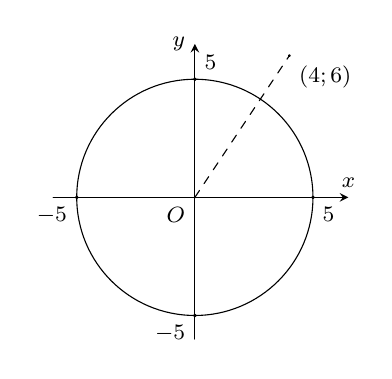
\begin{tikzpicture}[font=\footnotesize,line join=round, line cap=round, >=stealth,scale=0.3] 
			\draw[->] (-6,0)--(0,0)node[below left]{$O$} --(6.5,0)node[above]{$x$};
			\draw[->] (0,-6) -- (0,6.5) node[left]{$y$};
			\coordinate (O) at (0,0)  ;
			\coordinate (A) at (4,6);
			\fill (O) circle (1.5pt);
			\draw[fill=black] (A) circle (1pt) node [below right] {$(4;6)$};
			\draw (O) circle (5);
			\draw[dashed] (O)--(A);
			\draw[fill=black] (5,0) circle (1.5pt) node [below right] {$5$};
			\draw[fill=black] (-5,0) circle (1.5pt) node [below left] {$-5$};
			\draw[fill=black] (0,5) circle (1.5pt) node [above right] {$5$};
			\draw[fill=black] (0,-5) circle (1.5pt) node [below left] {$-5$};
		\end{tikzpicture}
}
	\shortans[oly]{2,21} %Chuẩn hóa ko quá 4 ký tự
	\loigiai{
		\begin{center}
			\begin{tikzpicture}[font=\footnotesize,line join=round, line cap=round, >=stealth,scale=0.5] 
				\draw[->] (-6,0)--(0,0)node[below left]{$O$} --(6.5,0)node[below]{$x$};
				\draw[->] (0,-6) -- (0,6.5) node[right]{$y$};
				\coordinate (O) at (0,0)  ;
				\coordinate (A) at (4,6);
				\draw[fill=black] (A) circle (1.5pt) node [below right] {$M(4;6)$};
				\draw (O) circle (5);
				\fill (O) circle (1.5pt);
				\draw[fill=black] (5,0) circle (1.5pt) node [below right] {$5$};
				\draw[fill=black] (-5,0) circle (1.5pt) node [below left] {$-5$};
				\draw[fill=black] (0,5) circle (1.5pt) node [above right] {$5$};
				\draw[fill=black] (0,-5) circle (1.5pt) node [below left] {$-5$};
				\draw[dashed] (O)--(A);
				\draw[fill=black] (2.75,4.18) circle (1.5pt) node [right] {$K$};
			\end{tikzpicture}
		\end{center}
		Gọi $M(4;6)$, $K$ là giao điểm của $OM$ và đường tròn.\\
		Khi đó khoảng cách ngắn nhất từ $M$ đến đường tròn là
		\begin{align*}
			MK=OM-OK=\sqrt{4^2+6^2}-5=\sqrt{52}-5\approx2{,}21.
		\end{align*}
	} 
\end{ex}
\begin{ex}[Trích đề thi HK2-THPT Nguyễn Khuyến-TPHCM-Năm học 2024-2025]%[0H9V4-7]%[Dự án đề cương 3 Khối NH25-26- Đợt 2- Nguyễn Cường]
	\immini{Hình vẽ bên dưới mô phỏng một trạm thu phát sóng điện thoại di động đặt ở vị trí $I$ có tọa độ $(-2;1)$ trong mặt phẳng tọa độ (đơn vị trên hai trục tọa độ là ki-lô-mét). Tính theo đường chim bay, xác định khoảng cách ngắn nhất để một người ở vị trí có tọa độ $(1;-1)$ di chuyển đến vùng phát sóng theo đơn vị ki-lô-mét (làm tròn kết quả đến hàng phần trăm), Biết rằng trạm thu phí được thiết kế với bán kính phát sóng là $3$ km.
	}
	{\begin{tikzpicture}[scale=0.8, line join=round, line cap=round, >=stealth, font=\footnotesize]
			\tikzset{every node/.style={scale=1}}
			\def\xmin{-5}\def\xmax{2}\def\ymin{-2}\def\ymax{4}
			\draw[->] (\xmin-0.2,0)--(\xmax+0.2,0) node[below left]{$x$};
			\draw[->] (0,\ymin-0.2)--(0,\ymax+0.2) node[right]{$y$};
			\draw (0,0) node[below left]{$O$};
			\clip (\xmin,\ymin) rectangle (\xmax,\ymax);
			\coordinate (I) at (-2,1);
			\coordinate (M) at (1,-1);
			\draw (I) circle(3cm) ($(I)+(0,0.5)$) node[above]{Trạm phát sóng};
			\draw[fill=black] (I) circle(1pt) node[above left]{$I$} (1,-1) circle(1pt) (-2,0) circle(1pt) node[below]{$-2$} (0,1) circle(1pt) node[right]{$1$} (1,0) circle(1pt) node[above]{$1$} (0,-1) circle(1pt) node[left]{$-1$};
			\draw[dashed] (-2,0)|-(0,1) (1,0)|-(0,-1);
		\end{tikzpicture}
	}
	\shortans[oly]{0,61}
	\loigiai{
		\immini{Gọi $M$ là vị trí của người ở vị trí $(1;-1)\Rightarrow M(1;-1)$.\\
			$A$ là điểm xa nhất mà có thể nhận được sóng điện thoại, suy ra điểm $A$ nằm trên đường tròn tâm $I(-2;1)$, bán kính $R=3$.\\
			Ta có $IM=\sqrt{(1+2)^2+(-1-1)^2}=\sqrt{13}$.\\
			Lại có $MA\ge |IM-IA|=\sqrt{13}-3$.\\
			Dấu \lq\lq$=$\rq\rq\, xảy ra khi và chỉ khi $3$ điểm $I$, $A$, $M$ thẳng hàng và $A$ nằm giữa $I$ và $M$.\\
			Vậy khoảng cách nhỏ nhất mà người đó di chuyển đến vùng phát sóng là $\sqrt{13}-3\approx 0{,}61$.
		}
		{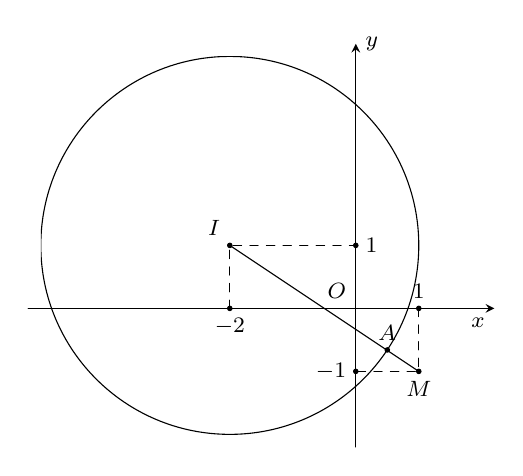
\begin{tikzpicture}[scale=0.8, line join=round, line cap=round, >=stealth, font=\footnotesize]
				\tikzset{every node/.style={scale=1}}
				\def\xmin{-5}\def\xmax{2}\def\ymin{-2}\def\ymax{4}
				\draw[->] (\xmin-0.2,0)--(\xmax+0.2,0) node[below left]{$x$};
				\draw[->] (0,\ymin-0.2)--(0,\ymax+0.2) node[right]{$y$};
				\draw (0,0) node[above left]{$O$};
				\clip (\xmin,\ymin) rectangle (\xmax,\ymax);
				\coordinate (I) at (-2,1);
				\coordinate (M) at (1,-1);
				\draw (I) circle(3cm) --(M);
				\draw[fill=black] (I) circle(1pt) node[above left]{$I$} (1,-1) circle(1pt) node[below]{$M$} (-2,0) circle(1pt) node[below]{$-2$} (0,1) circle(1pt) node[right]{$1$} (1,0) circle(1pt) node[above]{$1$} (0,-1) circle(1pt) node[left]{$-1$} (0.5,-0.66) circle(1pt) node[above]{$A$};
				\draw[dashed] (-2,0)|-(0,1) (1,0)|-(0,-1);
			\end{tikzpicture}
		}
	}
\end{ex}


\Closesolutionfile{ans}


\ind{PHẦN IV.} \inden{Tự luận.}\\
\setcounter{ex}{0}
\begin{ex}[Trích đề thi HK2-THPT Tân Châu-An Giang-Năm học 2024-2025]%[0H9N4-2]%[Dự án đề cương 3 Khối NH25-26- Đợt 2- Nguyễn Cường]
	Trong mặt phẳng $Oxy$, viết phương trình đường tròn có tâm $I(1;3)$ và đi qua điểm $M(3;1)$.
	\loigiai{
		$IM=\sqrt{(3-1)^2+(1-3)^2}=\sqrt{8}$.\\
		Đường tròn có tâm $I(1;3)$ và đi qua điểm $M(3;1)$, bán kính $R=IM=\sqrt{8}$ nên có phương trình là $$(x-1)^2+(y-3)^2=(\sqrt{8})^2\Leftrightarrow{(x-1)^2}+(y-3)^2=8.$$}
\end{ex}
\begin{ex}[Trích đề thi HK2- Bình Tân-TPHCM-Năm học 2024-2025]%[0H9H4-2]%[0H9H3-2]
	Trong mặt phẳng $Oxy$, cho $\triangle ABC$ có $A(1; 2)$, $B(-1; 1)$, $C(-2; 3)$.
	\begin{enumerate}
		\item Tìm toạ độ trọng tâm tam giác $ABC$.
		\item Viết phương trình đường thẳng chứa cạnh $AB$ của $\triangle ABC$.
		\item Viết phương trình đường tròn tâm $A$ và đi qua điểm $B$.
	\end{enumerate}
	\loigiai{
		\begin{enumerate}
			\item Tọa độ trọng tâm tam giác ${ABC}$ là ${G}\left(-\dfrac{2}{3} ; 2\right)$.
			\item
			Đường thẳng $A B$ đi qua $A(1 ; 2)$ và có vectơ chỉ phương $\vv{A B}=(-2 ;-1)$. Khi đó phương trình tham số của đường thẳng $AB$ là
			$\heva{&x=1-2t \\
				&y=2-t.}$
			\item Ta có $\vv{A B}=(-2 ;-1) \Rightarrow A B=\sqrt{5}$. \\
			Phương trình đường tròn tâm $A$, bán kính $AB$ là $(C)\colon (x-1)^{2}+(y-2)^{2}=5$.
		\end{enumerate}
}\end{ex}

\begin{ex}[Trích đề thi HK2- Bình Tân-TPHCM-Năm học 2024-2025]%[0H9V4-2]%[Dự án đề cương 3 Khối NH25-26- Đợt 2- Nguyễn Cường]
	Trong mặt phẳng $Oxy$, cho $A(2;-1)$, $B(0; 5)$; $C(-3; 7)$. Tìm tọa độ tâm đường tròn ngoại tiếp tam giác $ABC$.
	\loigiai{
		Gọi $M\left(x_{M} ; y_{M}\right)$ là tâm đường tròn ngoại tiếp tam giác ${ABC}$. Ta có:
		\allowdisplaybreaks
		\begin{eqnarray*}
			&&	\heva{
				{A M=B M} \\
				{A M=C M}
			} 
			\Leftrightarrow \heva{&A M^2=B M^2\\
				&A M^2=C M^2} \\
			&\Leftrightarrow&
			\heva{&\left(x_M-2\right)^2+\left(y_M+1\right)^2=x_M^2+\left(y_M-5\right)^2\\
				&\left(x_M-2\right)^2+\left(y_M+1\right)^2=\left(x_M+3\right)^2+\left(y_M-7\right)^2} \\
			&\Leftrightarrow& \heva{
				{-4x_{M}+12y_{M}=20} \\
				{-10x_{M}+16y_{M}=53}
			} \Leftrightarrow \heva{&x_M=-\dfrac{41}{7} \\
				&y_M=-\dfrac{2}{7}.}	
		\end{eqnarray*}
		Vậy $M\left(-\dfrac{41}{7} ;-\dfrac{2}{7}\right)$.
}\end{ex}

\begin{ex}[Trích đề thi HK2-THPT Nguyễn Thị Minh Khai-TPHCM-Năm học 2024-2025]%[0H9V4-5]%[Dự án đề cương 3 Khối NH25-26- Đợt 2- Nguyễn Cường]
	Trong mặt phẳng $Oxy$, cho đường tròn $(C)\colon x^2+(y-1)^2=1$ và $A(-2;0)$, $B(2;0)$. Tìm tọa độ điểm $M$ thuộc $(C)$ sao cho $MA+MB$ lớn nhất.
	\loigiai{
		Dễ thấy đường tròn $(C)$ đi qua $O(0;0)$.\\
		Giả sử điểm $M(x;y)$.\\
		Ta có 
		$$MA+MB\le \sqrt{2\left(MA^2+MB^2\right)}=\sqrt{2\left[(x+2)^2+y^2+(x-2)^2+y^2\right]}=\sqrt{4\left(x^2+y^2+4\right)}.$$
		\immini
		{
			Mà $x^2+y^2=MO^2\le (MI+IO)^2=4$.\\
			Vậy $MA+MB\le \sqrt{4(4+4)}=4\sqrt{2}$.\\
			Dấu bằng xảy ra khi $\heva{& MA=MB \\ & MO=2}\Rightarrow M(0;2)$.
		}
		{
			\begin{tikzpicture}[scale=1,>=stealth, font=\footnotesize, line join=round, line cap=round]
				\def\a{-1} \def\b{2} \def\c{2} % Hệ số
				\def\xmin{-2.5} \def\xmax{2.5}
				\def\ymin{-1} \def\ymax{3} 
				\draw[->] (\xmin,0)--(\xmax,0) node [below]{$x$};
				\draw[->] (0,\ymin)--(0,\ymax) node [left]{$y$};
				\node at (0,0) [below left]{$O$};
				\clip (\xmin+0.1,\ymin+0.1) rectangle (\xmax-0.1,\ymax-0.1);
				\path (-2,0) coordinate (A) (2,0) coordinate (B) (0,1) coordinate (I) ($(I)+(60:1)$) coordinate (M);
				\draw (I) circle (1cm);
				\draw (M)--(I) (M)--(0,0) (M)--(A) (M)--(B);
				\foreach \d/\g in {A/-90,B/-90,I/180,M/70} 
				\draw[fill=black] (\d) circle (1pt) +(\g:0.3) node{$\d$};
			\end{tikzpicture}
		}
	}
\end{ex}


\begin{ex}[Trích đề thi HK2 THPT Nguyễn Thị Minh Khai-TPHCM-Năm học 2024-2025]%[0H9V4-5]%[Dự án đề cương 3 Khối NH25-26- Đợt 2- Nguyễn Cường]
	Trong mặt phẳng $Oxy$, viết phương trình đường tròn đi qua $A(-8;-1)$ và tiếp xúc với đường thẳng $d\colon 3x+y+9=0$ tại $B(-4;3)$.
	\loigiai{
		Gọi $I$ là tâm của đường tròn, khi đó $IB\perp d$.\\
		Phương trình của đường thẳng $IB$ đi qua $B(-4;3)$ và vuông góc với $d$ là $x-3y+13=0$.\\
		Vì $IA=IB$ nên $I$ thuộc đường trung trực $\Delta$ của $AB$.\\
		Phương trình đường thẳng $\Delta$ qua $M(-6;1)$ là trung điểm của $AB$ và vuông góc với $AB$ là $x+y+5=0$.\\
		Tọa độ $I$ là nghiệm của hệ $\heva{& x-3y+13=0 \\ & x+y+5=0}\Leftrightarrow \heva{& x=-7 \\ & y=2.}\Rightarrow I(-7;2)$.\\
		Khi đó $R=IA=\sqrt{10}$.\\
		Vậy phương trình của đường tròn là $(x+7)^2+(y-2)^2=10$.
	}
\end{ex}
\begin{ex}[Trích đề thi HK2- Lê Quý Đôn- Hà Nội-Năm học 2024-2025]%[0H9H4-2]%[Dự án đề cương 3 Khối NH25-26- Đợt 2- Nguyễn Cường]
	Trong mặt phẳng $Oxy$, viết phương trình đường tròn có tâm nằm trên tia $Ox$ đồng thời đi qua gốc tọa độ và có bán kính bằng $2$.
	\loigiai{
		Gọi $I(x;0)$ $(x\leq0)$là tâm đường tròn.\\
		Đường tròn đi qua gốc tọa độ $O(0;0)$ và có $R=2$, suy ra $IO=R=\sqrt{x^2}=2 \Leftrightarrow \hoac{&x=2\\&x=-2.}$\\
		Do tâm $I$ nằm trên tia $Ox$ nên lấy $x=2$, suy ra tọa độ tâm là $I(2;0)$.\\
		Phương trình đường tròn với tâm $I(a;b)$ và bán kính $R$ có dạng $(x-a)^2+(y-b)^2=R^2$.\\
		Vậy phương trình đường tròn cần tìm là $(x-2)^2+y^2=4$.  
	}
\end{ex}

\begin{ex}[Trích đề thi HK2-THPT Nguyễn Thị Minh Khai-TPHCM-Năm học 2024-2025]%[0H9H4-3]%[Dự án đề cương 3 Khối NH25-26- Đợt 2- Nguyễn Cường]
	Trong mặt phẳng $Oxy$, viết phương trình tiếp tuyến của đường tròn $(C)\colon (x-1)^2+(y-3)^2=2$ vuông góc đường thẳng $d\colon x+y-2=0$.
	\loigiai{
		Đường tròn $(C)$ có tâm $I(1;3)$ và bán kính $R=\sqrt{2}$.\\
		Vì tiếp tuyến $\Delta$ vuông góc với đường thẳng $d$ nên $\Delta\colon x-y+c=0$.\\
		Ta có 
		$$\mathrm{d}(I,\Delta)=R\Leftrightarrow \dfrac{|c-2|}{\sqrt{2}}=\sqrt{2}\Leftrightarrow \hoac{& c=0 \\ & c=4.}$$
		Vậy $\Delta\colon x-y=0$ hoặc $\Delta\colon x-y+4=0$.
	}
\end{ex}

\begin{ex}[Trích đề thi HK2-THPT  Nguyễn Chí Thanh-TP HCM--Năm học 2024-2025]%[0H9H4-3]%[Dự án đề cương 3 Khối NH25-26- Đợt 2- Nguyễn Cường]
	Trong mặt phẳng $Oxy$, viết phương trình tiếp tuyến của đường tròn $(C) \colon x^2+y^2-4x+8y+10=0$ tại điểm $M(1;-1)$.
	\loigiai
	{
		\immini
		{
			Ta có $(C) \colon x^2+y^2-4x+8y+10=0 \Leftrightarrow (C) \colon (x-2)^2+ (y+4)^2= 10$.\\
			Do đó đường tròn $(C)$ có tâm là $I(2;-4)$.\\
			Gọi $\Delta$ là tiếp tuyến cần tìm.\\
			Ta có $\overrightarrow{IM}=(-1;3)$ là vectơ pháp tuyến của $\Delta$.\\
			Vậy phương trình đường thẳng $\Delta$ là
			\[
			-1\cdot (x-1)+3 \cdot (y+1)=0 \Leftrightarrow x-3y-4=0.
			\]
		}
		{
			\begin{tikzpicture}[>=stealth,line join=round,line cap=round,font=\footnotesize,scale=.61]
				\path 
				(2,-4) coordinate (I)
				(1,-1) coordinate (M)
				(-2,-2) coordinate (a)
				(3,-1/3) coordinate (b)
				;
				\draw (I) circle (3.16 cm);
				\draw (I)--(M) (a)--(b);
				\draw[fill=black] 
				(I) circle (1pt) node[below] {$I$}
				(M) circle (1pt) node[shift=(120:3mm)] {$M$}
				;
				\pic[draw,angle radius=2mm] {right angle=I--M--a};
				\path (a) node[above] {$\Delta$};
			\end{tikzpicture}
		}				
	}
\end{ex}

\begin{ex}[Trích đề thi HK2-THPT Trần Đại Nghĩa-TPHCM-Năm học 2024-2025]%[0H9V4-3]%[Dự án đề cương 3 Khối NH25-26- Đợt 2- Nguyễn Cường]
	Trong mặt phẳng $Oxy$, cho đường tròn $(C)\colon x^2+y^2-2 x+6 y-6=0$.  
	\begin{enumerate}
		\item Viết phương trình tiếp tuyến của $(C)$ biết rằng tiếp tuyến đó vuông góc với $\left(d_1\right)\colon-3 x+4 y-2024=0$
		\item Viết phương trình đường tròn $(C)$ đi qua hai điểm $A(0; 5)$, $B(2; 3)$ và có bán kính $R=\sqrt{10}$.
	\end{enumerate}
	\loigiai{
		\begin{enumerate}
			\item 
			Đường tròn $(C)$ có tâm $I(1;-3)$, bán kính $R=4$.\\
			Gọi $\Delta$ là tiếp tuyến của đường tròn.
			Vì tiếp tuyến $\Delta$ vuông góc với đường thẳng $\left(d_1\right)\colon-3 x+4 y-2024=0$ nên $\Delta$ có dạng $4x+3y+c=0$.\\
			$\Delta$ là tiếp tuyến của đường tròn $\Leftrightarrow \mathrm{d}(I,\Delta)=R \Leftrightarrow \dfrac{|4-9+c|}{\sqrt{4^2+3^2}}=4\Leftrightarrow |c-5|=20 \Leftrightarrow \hoac{&c=25\\&c=-15.} $\\
			Vậy có 2 phương trình tiếp tuyến thỏa mãn $\hoac{&4x+3y+25=0\\&4x+3y-15=0}$.
			\item 
			Gọi $I(a;b)$ là tâm đường tròn.\\
			Theo giả thiết ta có\\
			$IA=IB=R=\sqrt{10}\Leftrightarrow \heva{&IA^2=10\\&IA^2=IB^2}\Leftrightarrow \heva{&a^2+(b-5)^2=10\\&a^2+(b-5)^2=(a-2)^2+(b-3)^2}\Leftrightarrow\heva{&a^2+(b-5)^2=10 \quad(1)\\&b=a+3\quad(2).}$\\
			Thay (2) vào (1) ta được $a^2+(a-2)^2=10 \Leftrightarrow 2a^2-4a-6=0 \Leftrightarrow \hoac{&a=-1\Rightarrow b=2\\&a=3\Rightarrow b=6.}$\\
			\begin{itemize}
				\item Với $a=-1;b=2 \Rightarrow I(-1;2)$. Suy ra phương trình đường tròn $(C)\colon (x+1)^2+(y-2)^2=10$.
				\item Với $a=3;b=6 \Rightarrow I(3;6)$. Suy ra phương trình đường tròn $(C)\colon (x-3)^2+(y-6)^2=10$.
			\end{itemize}
			Vậy có 2 đường tròn thỏa mãn yêu cầu $\hoac{&(C)\colon (x+1)^2+(y-2)^2=10\\&(C)\colon (x-3)^2+(y-6)^2=10}$.
		\end{enumerate}
	}
\end{ex}

\begin{ex}[Trích đề thi HK2-THPT Phạm Văn Đồng-Khánh Hòa--Năm học 2024-2025]%[0H9V4-7]%[Dự án đề cương 3 Khối NH25-26- Đợt 2- Nguyễn Cường]
	Trên địa bàn huyện Khánh Vĩnh, đồn biên phòng có đặt một trạm thông tin tại vị trí có tọa độ $H(3;4)$ trong mặt phẳng tọa độ (đơn vị trên hai trục là ki-lô-mét). Biết trạm thông tin thu phát tín hiệu với bán kính phủ sóng $5$\,km. Trong đợt tuần tra, anh bộ đội bị thất lạc và không thể liên lạc được với đồn biên phòng. Tuy nhiên, theo thiết bị định vị anh đang ở vị trí có tọa độ $K(27;36)$. Anh đã di chuyển (theo đường chim bay) đoạn đường ngắn nhất tới vị trí có tọa độ $M(u;v)$ để có thể liên lạc với đồn biên phòng. Tính giá trị biểu thức $u^2+v^2+3{\,}424$.
	\loigiai{\begin{center}
			\begin{tikzpicture}[line join=round, line cap=round, thick, scale=0.5]
				%hidden: VM019
				\path 
				(0,0) coordinate (H)
				++(30:2) coordinate (M)
				($(H)!8!(M)$) coordinate (K)
				;
				\draw (K)node{\Huge \faStreetView}node[shift={(0,-.8)}]{$K$}--(H)node[below]{$H$} (M)node[right]{$M$};
				\draw[dashed] (H)circle (2);
				\fill (M) circle(2pt);
				\fill (K) circle(2pt);
				\node at (0,0){\href{1JAECB}{\tiny \phantom{1JAECB}}};
			\end{tikzpicture}
		\end{center}
		Phương trình đường tròn mô tả ranh giới bên ngoài của vùng phủ sóng là $(C) \colon (x-3)^2+(y-4)^2=25$.\\
		Ta có $\overrightarrow{KM}=(u-27;v-36)$,  $\overrightarrow{KH}=(-24;-32)$ và
		\[KH=\sqrt{(-24)^2+(-32)^2}=40\;\mathrm{km}.\]
		Điểm $K$ nằm ngoài đường tròn $(C)$ nên khoảng cách ngắn nhất từ người đứng ở vị trí $K$ đến vùng phủ sóng là 
		\[KM=KH-R=40-5=35\;\mathrm{km}.\]
		Vì $M$ là giao điểm của đường thẳng $KH$ và đường tròn $(C)$ nên $\overrightarrow{KM}$ cùng phương với $\overrightarrow{KH}$ và $\dfrac{KM}{KH}=\dfrac{35}{40}=\dfrac{7}{8}$.\\
		Khi đó tọa độ điểm $M$ thỏa mãn
		\[\overrightarrow{KM} =\dfrac{7}{8} \cdot \overrightarrow{KH} \Leftrightarrow \heva{&u-27=\dfrac{7}{8} \cdot(-24)  \\&v-36=\dfrac{7}{8} \cdot (-32)} \Leftrightarrow \heva{&u= 6\\&v=8.}\]
		Suy ra $M(6;8)$.\\
		Vậy $u^2+v^2+3{\,}424=3{\,}524$.
	}
\end{ex}

